\documentclass[a4paper,oneside,openright,spanish,english]{book}
\usepackage[paperwidth=18cm,margin=2cm]{geometry}
\usepackage{emptypage}
\usepackage{layouts}
\printinunitsof{cm}
\usepackage{graphicx}
\usepackage[square,sort,comma,numbers]{natbib}
\usepackage{amsmath}
\usepackage{amssymb}
\usepackage{amsfonts}
\usepackage{float}
\usepackage{caption}
\usepackage{wasysym}
\usepackage{tikz}
\usepackage{float}
\usepackage{subcaption}
\usepackage{nameref}
%\usepackage{fixmath}
\usepackage{makecell}
\usepackage[toc,page]{appendix}
\usepackage{longtable}
\usepackage{cprotect}
\usepackage{cleveref}
\usepackage{gensymb}
\usepackage{bm}
\usepackage{comment}
\usepackage{breqn}
\usepackage{mathtools}
\newenvironment{spmatrix}[1]
 {\def\mysubscript{#1}\mathop\bgroup\begin{pmatrix}}
 {\end{pmatrix}\egroup_{\textstyle\mathstrut\mysubscript}}
\DeclareMathOperator{\Tr}{Tr}
\DeclareMathOperator{\spn}{span}
\newcommand{\minus}{\scalebox{0.75}[1.0]{$-$}}
\geometry{bindingoffset=2cm}
\geometry{textwidth=345pt}
\usepackage{url}
\def\UrlBreaks{\do\/\do-}

\begin{document}

\pagenumbering{roman}
\graphicspath{{images/}}

\begin{titlepage}
\title{Discontinuous Galerkin method for direct numerical simulation of the Stokes equation}
\author{Nirav Vasant Shah, \\M.Sc. Water Resources Engineering and Management, \\Universit\"at Stuttgart, \\Stuttgart, Germany\\ 
\and Home supervisor: Prof. Dr. Bernard Haasdonk,\\ Institute of Applied Analysis and Numerical Simulation, \\Universit\"at Stuttgart,\\ Stuttgart, Germany\\ \and Host supervisor: Prof. Dr. Gianluigi Rozza,\\ SISSA, Scuola Internazionale Superiore di Studi Avanzati, \\Mathematics area, mathlab, \\Trieste, Italy \\ \and Host supervisor: Dr. Martin Hess,\\ SISSA, Scuola Internazionale Superiore di Studi Avanzati, \\Mathematics area, mathlab,  \\Trieste, Italy }
\date{\today}
\maketitle

\end{titlepage}

\tableofcontents
\newpage

\chapter[Perspective and formulation]{Engineering perspective and mathematical formulation} 

The importance of the Navier-Stokes equations is impossible to be ignored as far as mathematical approaches in fluid mechanics are concerned. The subject of mathematical applications in fluid mechanics starts with  one of the variants of the Navier-Stokes equations, such as the Stokes equation. Almost all processes of fluid mechanics require considerations related to the Navier-Stokes equations. Navier-Stokes equation is non-linear, characterizing flow fluctuations. As the incompressible condition is imposed the state variables are constant. However, in case of laminar flow, i.e. when fluctuations are negligible. This linearized form of the Navier-Stokes equation is the Stokes equation.

\section[Derivation]{Derivation of the Navier-Stokes and Stokes equations}

Before deriving the Navier-Stokes equations we introduce some notations. The domain is denoted by $\Omega \subseteq \mathbb{R}^d $. The domain boundary is denoted by $\partial \Omega$. The domain boundary is divided into Dirichlet boundary $\Gamma_D$ and Neumann boundary $\Gamma_N$ i.e. $\Gamma_D \cup \Gamma_N = \partial \Omega $, $\Gamma_D \cap \Gamma_N = \emptyset $. 

The governing equations for the incompressible Navier-Stokes flows are the conservation equations: Mass conservation and Momentum conservation. The conservation equations are derived based on the concept of control volume and the control surface. The control volume is the volume, fixed or moving with constant velocity in space, through which the fluid moves. Extensive quantity is the amount of a quantity contained in the system such as mass. Extensive quantity when measured per unit mass, is called intensive quantity. For example, extensive quantity momentum corresponds to the intensive quantity velocity, momentum per unit mass. Intensive quantity is independent of the mass of the system and is not additive, while extensive quantity does depend on the mass of the system and is additive. The control surface is the surface enclosing the control volume. All equations can be derived from the Reynold's transport equation as presented for example by White F.M. \cite{white}:


\begin{equation} \label{rtt} 
\frac{dB'}{dt'}|_{cs} = \frac{d}{dt'} \int_{cv} b' \rho dV + \int_{cs} (b' \rho) u\cdot dA 
\end{equation}
{}\\
$cv$ = Control volume,\\
$cs$ = Control surface,\\
$B'$ = Extensive quantity under consideration,\\
$b'$ = Intensive quantity corresponding to $B'$,\\
$\rho$ = Density of fluid,\\
$u$ = Velocity of fluid.\\

If in the above equation $B'$ is substituted as momentum $M$ and correspondingly $b'$ as velocity $u$, we obtain the change in momentum. As per Newton's second law of motion change in momentum is equal to the sum of external forces acting on the system. 

\begin{equation}\label{External force lhs}
F = \frac{dM}{dt'} = \frac{d}{dt'} \int_{cv} u \rho dV + \int_{cs} (u \rho) u\cdot dA \textrm{.}
\end{equation}

This sum of forces arises from stresses $\sigma$ (shear stresses and normal stresses) and external force $f$ such as weight. 

\begin{equation}\label{External force rhs}
F = \int_{cs} \sigma \cdot dA + \int_{cv} \rho f dV \textrm{,}
\end{equation}
\\
$\sigma =$ Viscous stress,\\
$f =$ External force per unit volume.\\

Equating external forces with change in momentum i.e. equating \eqref{External force lhs} and \eqref{External force rhs}, considering steady conditions only, using definition of viscous stress tensor and with the application of the Gauss divergence theorem we arrive at the Navier Stokes equation,

\begin{equation} \label{navier_stokes}
-2\nabla \cdot (\nu \nabla^s u) + (1/\rho) \nabla p + (u \cdot \nabla)u = f \quad   \textnormal{in}  \quad \Omega \textrm{.}
\end{equation} 

The incompressible mass conservation equation can be derived similarly by substituing $B' =$ Mass of control system and $b' = 1$ in equation \eqref{rtt}.  It can be written as,

\begin{equation}\label{mass_conservation}
\nabla \cdot u=0 \quad   \textnormal{in}  \quad \Omega \textrm{.}
\end{equation}

The boundary conditions are expressed as,\\

Dirichlet boundary:
\begin{equation}\label{dirichlet_ns}
u=u_D \quad \textnormal{on} \quad \Gamma_D \textrm{.}
\end{equation}

Neumann boundary:
\begin{equation} \label{neumann_ns}
-pn + 2\nu(n \cdot \nabla^s)u = t \quad   \textnormal{on}  \quad \Gamma_N \textrm{.}
\end{equation}

$ $\\
$u$ = flow velocity and $u:\Omega \rightarrow \mathbb{R}^d$,\\
$p$ = pressure and $p:\Omega \rightarrow \mathbb{R}$,\\
$\nu$ = kinematic viscocity (fluid property) and $\nu:\Omega \rightarrow \mathbb{R}$,\\ 
$\rho$ = density (fluid property) and $\rho:\Omega \rightarrow \mathbb{R}$,\\
$f$ = external force and $f:\Omega \rightarrow \mathbb{R}^d$,\\
$u_D$ = specified flow velocity at Dirichlet boundary and $u_D:\Gamma_D \rightarrow \mathbb{R}^d$,\\
$n$ = normal unit vector and $n:\partial \Omega \rightarrow \mathbb{R}^d$,\\
$t$ = specified Neumann flux and $t:\Gamma_N \rightarrow \mathbb{R}^d$.\\

\begin{center}
$\nabla^s = \frac{1}{2}(\nabla + \nabla^T) \textrm{.}$
\end{center}

The equation \eqref{navier_stokes} is known as the strong form of the momentum conservation of the Navier Stokes equation.

It can be seen that the steady state Navier Stokes equation is nonlinear and has two unknown variables, pressure $p$ and velocity $u$. The additional equation, mass conservation equation, is hence necessary to obtain a sufficient number of equations for the number of unknowns.

We also introduce the dimensionless number Reynolds number, $Re$ which is the most characteristic quantity of the flow. The Reynolds number is defined as the ratio of inertial force to the viscous force,

\begin{equation} \label{reynolds_number}
Re = \frac{uL}{\nu} \textrm{.}
\end{equation}

Where, $L$ is the characteristic geometrical dimension, such as the diameter of a pipe in case of pipe flow or the span of the wing of an aircraft in case of flow over an aircraft wing.\\

\section{Direct numerical simulation} 

We now differentiate between the type of flows, laminar and turbulent.\\

Laminar flow is characterised by well defined velocity and pressure field and low Reynolds number. This flow has very low velocity fluctuations and pressure fluctuations. The viscous force is balanced by the pressure force and the flow has negligible inertial force. Mathematically, the non linear term in \eqref{navier_stokes} is no longer present. This equation is known as Stokes equation (White F.M.\cite{white}).\\

The strong form of the Stokes equation is as follow,

\begin{equation} \label{stokes_strong_form}
-\nu \Delta u + \nabla p = f \quad \textrm{in} \quad \Omega \textrm{,}
\end{equation}

\begin{equation} \label{dirichlet condition stokes}
u = u_D \quad \textrm{on} \quad \Gamma_D \textrm{,}
\end{equation}

\begin{equation} \label{neumann condition stokes}
-pn + \nu n \cdot \nabla u = t \quad \textrm{on} \quad \Gamma_N \textrm{.}
\end{equation}
\\

Turbulent flow, in contrast, is characterised by fluctuations in velocity and pressure field and a high Reynolds number. The flow has high velocity and an inertial force is present in addition to a viscous and a pressure force. This inertial force makes the Equation \eqref{navier_stokes} non linear. The fluctuations of velocity and pressure are of the order of the Kolmogrov scale (Kundu et al. \cite{Kundu}).\\

We now discuss, in next chapter, about the grid formation, deriving and solving weak formulation from the strong formulation presented in this chapter of the Stokes equation.


\chapter[DG formulation for the Stokes equation]{Discontinuous Galerkin formulation for Stokes equation}

\section{Grid geometry}

In numerical analysis a continuous problem is posed over finite number of degrees of freedom. We divide the original domain into smaller subdomains to have finite number of degrees of freedom. The divided domain is called grid. If the original domain is denoted by $\Omega$, we denote the grid by $\mathcal{T}$. In the present case, we use triangular grid and denote each triangle as $\tau_k$ with $k$ as element index. If $nel$ is the total number of elements in the grid, $1\leq k \leq nel$. We note that $\mathcal{T} = \cup_{k=1}^{nel} \tau_k$. Each triangle is an 'Element' of the grid. The boundary between elements i.e. interelement boundary is denoted by $\Gamma$. In case of a grid, the boundary $\partial \mathcal{T}$ comprises of domain boundaries and interelement boundaries i.e. $\partial \mathcal{T} = \Gamma_D \cup \Gamma_N \cup \Gamma$. During discussion on jump operator and average operator we denote the element under consideration as $\tau_{h}^+$ and neighbouring element as $\tau_{h}^-$ (Figure \ref{fig:Self_neighbour}).

\begin{figure}
\centering
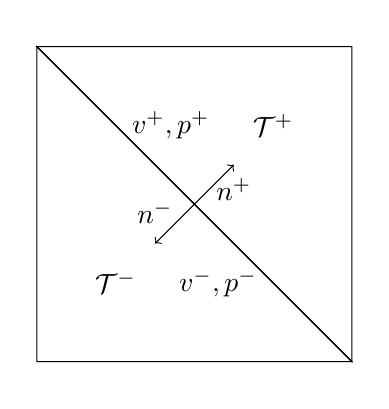
\begin{tikzpicture}
\draw (0,0) node[anchor=north]{${}$}
  -- (4,0) node[anchor=north]{${}$}
  -- (0,4) node[anchor=south]{${}$}
  -- cycle;
\draw (4,4) node[anchor=north]{${}$}
  -- (4,0) node[anchor=north]{${}$}
  -- (0,4) node[anchor=south]{${}$}
  -- cycle;
\draw[->] (2,2)--(2.5,2.5)node[label={[xshift=0cm, yshift=-0.7cm]${n^+}$}]{};
\draw[->] (2,2)--(1.5,1.5)node[label={[xshift=0cm, yshift=0cm]${n^-}$}]{};
\node at (1,1){$\mathcal{T^-}$};
\node at (3,3){$\mathcal{T^+}$};
\node at (1.7,3){$v^+,p^+$};
\node at (2.3,1){$v^-,p^-$};
\end{tikzpicture}
\caption{Element self (+) and neighbouring element (-)}
\label{fig:Self_neighbour}
\end{figure}

we introduce $\mathbb{M}$ as the space of unit normals to boundaries of $\Omega$. We also denote the normal pointing from element itself towards neighbouring element as $n^+ \in \mathbb{M}$ and the normal pointing from neighbouring element towards element itself as $n^- \in \mathbb{M}$, such that $n^+ = - n^-$. Correspondingly every quantity on element itself is denoted by superscript $+$ and on neighbouring element is denoted by $-$.  We denote by $h_{\tau_k}$ the diameter of element $\tau_k$ such that $h_{\tau_k} = \sup ||x-y||$ where, $(x,y) \in \tau_k$. We also denote by $\theta_k$ the smallest angle of the element $\tau_k$.

In case of a 2-dimensional domain the grid could be a triangular grid or a rectangular grid. The triangular grids are useful for irregular geometry and also on regular geometry if the solution is expected to be irregular due to complex flow physics. This flexibility requires additional efforts to define the grid accurately. That is, unlike a structured grid, an unstructured grid needs to define connectivity of vertices, which form edges, which in turn form a face. In case of a 2-dimensional grid we have faces which are 2-dimensional entities, edges which are 1-dimensional entities and points or vertices which are 0-dimensional entities. In case of 3-dimensional grid, these faces constitute tetrahedral elements. 

\section{Grid parameters}

We refer to 'Grid parameters' as the geometrical parameters which are dependent on the geometry of the problem or the grid or both. These parameters do not depend upon the mathematical formulation but are supplementary to the mathematical formulation. On the triangular grid we have 3 entities: faces, edges, vertices as explained above. From faces we have the area (equivalent to volume of element in case of a 3-dimensional grid) and the Jacobian. As explained later in the weak form of the Stokes and Navier-Stokes Discontinuous-Galerkin formulation and transformation between local and global geometry, the area of element is useful for volume integral terms and the Jacobian is useful for transformation between local and global geometry. From edges we derive the edge length $l$ which is useful for boundary integral terms and normal vector $n$ which is useful for flux calculation. The normal vector is the unit vector normal to the edge pointing outward from the element. Every element has 3 neighbouring elements and the element shares each of his edge with one of its neighbour. From vertices we derive the vertex index which helps to define the connectivity of the vertices which is useful especially in case of unstructured grid. In order to give clear visualization of continuous domain and grid, we refer to Figure \ref{fig:continuous_grid_figure}.

\begin{figure}[H]
\begin{subfigure}{0.5\textwidth}
\centering
  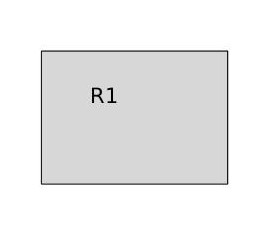
\includegraphics[width=\linewidth]{domain.jpg}
  \label{fig:Domain}
\end{subfigure}
\begin{subfigure}{0.5\textwidth}	
\centering
  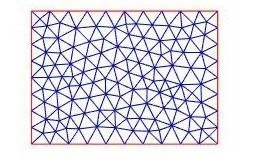
\includegraphics[width=\linewidth]{grid.jpg}
  \label{fig:Mesh}
\end{subfigure}
\caption{Continuous domain (left) and discretised domain or grid (right)}
\label{fig:continuous_grid_figure}
\end{figure}

\section{Jump operator} \label{jump_operator_ch3}

The jump operator of a quantity $[u]$ at an internal boundary is defined as,
\begin{equation}\label{jump operator}
[u]=u^+ \cdot n^+ + u^- \cdot n^- \textrm{,}
\end{equation}

where $n$ is the unit normal to an edge of an element pointing outward from the element.

As pointed out by Montlaur et al. \cite{Montlaur2} this jump representation has two disadvantages.\\
\noindent
1. The function space of the quantity itself and the function space of the jump are different that is, the jump of a vector is scalar and jump of a scalar is vector.\\
2. The use of this definition camouflages the presence of a normal.\\

To overcome these disadvantages Montlaur et al. \cite{Montlaur2} modified jump representation as below :\\

1.  For scalar quantity $p$,
\begin{equation}
\begin{split}
[pn] = p^+ n^+ + p^- n^- \quad \textrm{on} \quad \Gamma \textrm{,}\\
[pn] = p n \quad \textrm{on} \quad \Gamma_D \textrm{.}
\end{split}
\end{equation}

2. For vector quantity $u$ ($n \otimes u = u_i n_j$, $1 \leq i \leq d_u$, $1 \leq j \leq d$),
\begin{equation}
\begin{split}
[n \otimes u] = n^+ \otimes u^+ + n^- \otimes u^- \quad \textrm{on} \quad \Gamma \textrm{,}\\
[n \otimes u] = n \otimes u \quad \textrm{on} \quad \Gamma_D \textrm{,}\\
 \textrm{or} \\
[n \cdot u] = n^+ \cdot u^+ + n^- \cdot u^- \quad \textrm{on} \quad \Gamma \textrm{,}\\
[n \cdot u] = n \cdot u \quad \textrm{on} \quad \Gamma_D \textrm{.}\\
\end{split}
\end{equation}

As can be seen the quantity and its jump are now in same space i.e. jump of vector is vector and jump of scalar is scalar.

\section{Average operator}

The average operator is defined as :

\begin{equation}\label{average operator}
\left\lbrace u \right\rbrace = \frac{u^+ + u^-}{2} \textrm{.}
\end{equation} 
\noindent
As can be seen definition of average operator does not involve normal and hence, is simpler as compared to the Jump operator.\\
Also, $u$ and $\lbrace u \rbrace$ are in same function space i.e. average of a vector is vector and average of scalar is scalar.\\

\section{$L^2$ scalar product}

We denote the $L^2$ scalar product of $p$ and $q$ by $(p,q)$ as below :\\

If $p$ and $q$ are scalars,
\begin{equation}\label{inner product scalars}
(p,q)=\int_{\Omega} pq \textrm{.}
\end{equation}

If $p$ and $q$ are vectors,
\begin{equation}\label{Inner product vectors}
(p,q)=\int_{\Omega} p \cdot q \textrm{.}
\end{equation}

If $p$ and $q$ are tensors,
\begin{equation}\label{Inner product tensors}
(p,q)=\int_{\Omega} p : q \quad \textrm{where} \quad p:q = Tr(pq^T) \textrm{.}
\end{equation}

\section{Discontinuous-Galerkin (DG) method}

In the context of the discontinuous Galerkin method we introduce the function spaces $V$($\mathcal{T}$) and $Q$($\mathcal{T}$) for analytical solution of velocity and analytical solution of pressure respectively. The space containing high fidelity solution (in this case discontinuous Galerkin) is called truth space denoted by $\mathbb{V}$ for velocity and $\mathbb{Q}$ for pressure. $d_u$ and $d_p$ represent the dimension of velocity and pressure respectively.

\begin{equation} \label{velocity_test}
\mathbb{V} = \lbrace \phi \in (L^2(\mathcal{T}))^{d_u}| \quad \phi \in (P^D(\tau_k))^{d_u} \quad \forall \quad {\tau_k} \in \mathcal{T} \rbrace
\end{equation}

\begin{equation} \label{pressure_test}
\mathbb{Q} = \lbrace \psi \in (L^2(\mathcal{T}))^{d_p}| \quad \psi \in (P^{D-1}(\tau_k))^{d_p} \quad \forall \quad {\tau_k} \in \mathcal{T} \rbrace
\end{equation}

Here, $P^D(\tau_k)$ denotes space of polynomials of degree at most $D$ over $\tau_k$.\\

We apply a similar procedure as in the finite element method i.e. multiplying the partial differential equation by a test function and integration by parts (Section \ref{Stokes_flow_ch3}). However, we note that our test function is not continuous on the interface. Hence, we require flux approximations and jumps at the interface. These requirements have given rise to different discontinuous Galerkin methods. For explanation of each method we refer to literatures such as by Persson et al. \cite{persson} for local discontinuous Galerkin method and by Montlaur et al. \cite{Montlaur} for the Compact discontinuous Galerkin method and the Interior penalty method. \\

Discontinuous-Galerkin methods for the Navier Stokes equation were compared by Montlaur et al. \cite{Montlaur}. The local discontinuous Galerkin (LDG) method extends the computational stencil beyond immediate neighbours whereas compact discontinuous Galerkin (CDG) and interior penalty method (IPM) only connect to neighbouring elements. The CDG method provides more flexibility with respect to the stabilisation constant at the cost of additional simulation effort related to computation of the lifting operator, while the IPM method requires restrictions on penalty parameter in order to maintain coercivity of bilinear form. However, implemenetation of IPM is simpler as compared to implementation of CDG. Both methods, CDG and IPM, have almost similar convergence rates. 

\section{Stokes strong, weak and discrete form} \label{Stokes_flow_ch3}

The strong form of the Stokes equation is as follow,

\begin{equation} \label{stokes_strong_form_ch3}
-\nu \Delta u + \nabla p = f \quad \textrm{in} \quad \Omega \textrm{.}
\end{equation}

\begin{equation} \label{dirichlet condition stokes_ch3}
u = u_D \quad \textrm{on} \quad \Gamma_D \textrm{.}
\end{equation}

\begin{equation} \label{neumann condition stokes_ch3}
-pn + \nu n \cdot \nabla u = t \quad \textrm{on} \quad \Gamma_N \textrm{.}
\end{equation}


\subsubsection{Derivation of the weak form of the Stokes equation} \label{derivation_weak_stokes}

We multiply the equation \eqref{stokes_strong_form_ch3} by $\phi$ and integrate over $\mathcal{T}$,
\begin{equation}
\int_{\mathcal{T}} (- \phi \nu \Delta u + \phi \cdot \nabla p) = \int_{\mathcal{T}} \phi \cdot f \textrm{.}
\end{equation}

By applying Gauss divergence theoreom,
\begin{equation}
\int_{\mathcal{T}} (-\nabla (\phi \nu \nabla u) + (\nu \nabla \phi : \nabla u) + \nabla \cdot (p \phi) - (p \nabla \cdot \phi)) = \int_{\mathcal{T}} \phi \cdot f \textrm{,}
\end{equation}

\begin{equation}
\int_{\Gamma \cup \Gamma_D \cup \Gamma_N} (- [(\phi \nu \nabla u)] + \int_{\mathcal{T}}  (\nu \nabla \phi : \nabla u) + \int_{\Gamma \cup \Gamma_D \cup \Gamma_N}  [p \phi] - \int_{\mathcal{T}}  (p \nabla \cdot \phi)) = \int_{\mathcal{T}} \phi \cdot f \textrm{.}
\end{equation}

Following symmetric formulation for jump operator proposed by Peraire et al. \cite{peraire},
\begin{equation}
\int_{\Gamma \cup \Gamma_D \cup \Gamma_N} [(\phi \nu \nabla u)] = \int_{\Gamma} (\lbrace \phi \rbrace : [n \otimes \nabla u]) + \int_{\Gamma} (\lbrace \nabla u \rbrace : [n \otimes \phi]) + \int_{\Gamma_D \cup \Gamma_N} (\phi \cdot u ) \textrm{,}
\end{equation}

and 

\begin{equation}
\int_{\Gamma \cup \Gamma_D \cup \Gamma_N} [p \phi] = \int_{\Gamma} (\lbrace p \rbrace [ n \cdot \phi]) + \int_{\Gamma} (\lbrace \phi \rbrace \cdot [pn]) + \int_{\Gamma_D \cup \Gamma_N} (p (n \cdot \phi) ) \quad \textrm{.}
\end{equation}

It is to be noted that analytical solution is continuous and hence $[u] = 0$. Therefore we add the term $([u],[\phi])$ which helps to maintain the coercivity of discontinuous approximation.


Collecting all Neumann boundary integral terms, the weak form of Stokes equation is as follow,

\begin{equation}\label{stokes_weak_ch3}
\begin{split}
a_{IP}(u,\phi) + b(\phi,p) + (\lbrace p \rbrace,[n\cdot \phi])_{\Gamma \cup \Gamma_D} = l_{IP}(\phi) \ .
\end{split}
\end{equation}

\begin{equation}\label{a_IP}
\begin{split}
a_{IP}(u,\phi) = (\nabla u, \nabla \phi) + C_{11} ([n \otimes u],[n \otimes \phi])_{\Gamma \cup \Gamma_D} \\
- \nu (\{\nabla u\},[n \otimes \phi])_{\Gamma \cup \Gamma_D} - \nu ([n \otimes u],\{\nabla \phi\})_{\Gamma \cup \Gamma_D} \textrm{.}
\end{split}
\end{equation}

It is to be noted that penalty paramter $C_{11}$ is to be kept large enough to maintain coercivity of bilinear form.

\begin{equation}\label{b}
b(\phi,\psi) = -\int_{\mathcal{T}} \psi \nabla \cdot \phi \ ,
\end{equation}

\begin{equation}\label{l_IP}
\begin{split}
l_{IP}(\phi) = (f,\phi) + (t,\phi)_{\Gamma_N} + C_{11} (u_D,\phi)_{\Gamma_D} - (n \otimes u_D, \nu \nabla \phi)_{\Gamma_D} \ .
\end{split}
\end{equation}

\begin{itemize}
\item We refer to the term $(\lbrace p \rbrace,[n\cdot \phi])_{\Gamma \cup \Gamma_D}$ as ``pressure flux term".
\item $b(\phi,\psi)$ represents the ``incompressibility term".
\item We call $(f,\phi)$ as the ``source term".
\item We refer to $(t,\phi)_{\Gamma_N}$ as the ``Neumann boundary term".
\item The terms $C_{11} (u_D,\phi)_{\Gamma_D}$, $(n \otimes u_D, \nu \nabla \phi)_{\Gamma_D}$ are referred to as the ``Dirichlet boundary terms".
\end{itemize}

The discrete form of Stokes equation is written as,

\begin{equation} \label{stokes discrete_ch3}
AU + BP = F_1 \textrm{.}
\end{equation}

Matrix $A$ and matrix $B$ are calculated as per equation \ref{matrix A} and equation \ref{matrix B} respectively. \\

The strong form of continuity equation is as follow,

\begin{equation}
\nabla \cdot u = 0 \quad \textrm{in} \quad \Omega \textrm{.}
\end{equation}

and the weak for of continuity equation is as follow,

\begin{equation}\label{contiuity_weak_ch3}
\begin{split}
b(u,\psi) + (\{\psi\},[n\cdot u])_{\Gamma \cup \Gamma_D} = (q,n\cdot u_D)_{\Gamma_D} \textrm{.}
\end{split}
\end{equation}

The discrete form of continuity equation is written as,

\begin{equation} \label{continuity discrete_ch3}
B^T U  = F_2 \textrm{.}
\end{equation}

Discrete form of equations can be written in Matrix form as, 

\begin{equation} \label{Stokes_matrix_ch3}
\begin{spmatrix}{\textrm{Stiffness matrix}}
    A & B \\
    B^T & 0
\end{spmatrix}
\begin{spmatrix}{\textrm{Solution vector}}
    U \\
    P
\end{spmatrix}
=
\begin{spmatrix}{\textrm{Right hand side (Known)}}
    F_1  \\
    F_2
\end{spmatrix}
\textrm{.}
\end{equation}

Here, $(\cdot , \cdot)$ is $L^2$ inner product, $\{\cdot\}$ is average operator, $[\cdot]$ is jump operator. 

\subsection{Properties of the stiffness matrix} \label{property_stif_mat_stokes}

We now write each element of matrix $A$. We represent components of Unit normal vector as $n = [n_1 \quad ... \quad n_d]$.

\begin{equation} \label{matrix A}
\begin{split}
A_{ij} = \sum_{k=1}^d (\frac{\partial \phi_i}{\partial x_k} , \frac{\partial \phi_j}{\partial x_k}) + \sum_{k=1}^d C_{11} ([\phi_i n_k] , [\phi_j n_k])_{\Gamma \cup \Gamma_D} \\ - \sum_{k=1}^d \nu ([\phi_i n_k] , \lbrace \frac{\partial \phi_j}{\partial x_k} \rbrace)_{\Gamma \cup \Gamma_D} - \sum_{k=1}^d \nu (\lbrace \frac{\partial \phi_i}{\partial x_k} \rbrace , [\phi_j n_k])_{\Gamma \cup \Gamma_D} \ .
\end{split}
\end{equation}
${}$\\

\begin{itemize}

\item We call the term $(\frac{\partial \phi_i}{\partial x_k} , \frac{\partial \phi_j}{\partial x_k})$ as ``diffusive term" as it represents diffusion of momentum from strong formulation. 
\item We call the term $C_{11} ([\phi_i n_k] , [\phi_j n_k])_{\Gamma \cup \Gamma_D} \\ - \nu \sum_{k=1}^d ([\phi_i n_k] , \lbrace \frac{\partial \phi_j}{\partial x_k} \rbrace)_{\Gamma \cup \Gamma_D}$ as the ``coercivity term" as this term helps to ensure coercivity of the $a_{IP}$ (equation \eqref{a_IP}). 
\item We refer to the term $\nu ([\phi_i n_k] , \lbrace \frac{\partial \phi_j}{\partial x_k} \rbrace)_{\Gamma \cup \Gamma_D}$ (or $\nu (\lbrace \frac{\partial \phi_i}{\partial x_k} \rbrace , [\phi_j n_k])_{\Gamma \cup \Gamma_D}$) as ``flux approximation" since it represents approximation of flux at the internal or domain boundary.

\end{itemize}

We can see following properties of $A$: 
\\
1. $A_{ij} = A_{ji} \implies$ Symmetric,\\
2. $A$ is positive definite : As the penalty parameter $C_{11}$ is adjusted to ensure coercivity of $A$,\\
$\exists \quad c' > 0 $ and for any non zero vector $z$,
\begin{equation}
z^T A( \phi , \phi ) z \geq c' || z ||^2 \implies z^T A( \phi , \phi ) z > 0 \textrm{.}
\end{equation}
3. Size of matrix $A$: $A \in \mathbb{R}^{u_{ndofs} \times u_{ndofs}}$ ($u_{ndofs}$ is the total number of degrees of freedom of velocity).\\

Each element of $B$ can be represented as,\\
\begin{equation} \label{matrix B}
B_{ij} = - \int_{\mathcal{T}} \frac{\partial \phi_i}{\partial x_i} \psi_j +
(\lbrace \psi_j \rbrace , [n \cdot \phi_i])_{\Gamma \cup \Gamma_D} \ .
\end{equation}

We notice that, Size of matrix $B$: $B \in \mathbb{R}^{u_{ndofs} \times p_{ndofs}}$ ($p_{ndofs}$ is total number of degrees of freedom of pressure)

$u_{ndofs}$ and $p_{ndofs}$ i.e. total number of degrees of freedom of velocity and pressure respectively on triangular grid and taylor-hood pressure velocity basis function can be calculated as below. In present analysis we have $d_u = 2$ and $d_p = 1$ and we represent total number of elements as $nel$.

\begin{equation} \label{undofs}
u_{ndofs} = 2 \quad \left( \frac{(D+1)(D+2)}{2} \right) \quad nel
\end{equation}

\begin{equation} \label{pndofs}
p_{ndofs} = \left(\frac{D(D+1)}{2}\right) \quad nel
\end{equation}

With above considerations we arrive at following conclusions, \\
${}$\\
1. Stiffness matrix is symmetric, \\
2. Stiffness matrix $ \in \mathbb{R}^{(u_{ndofs} + p_{ndofs}) \times (u_{ndofs} + p_{ndofs})}$,\\
3. The number of positive eigenvalues of stiffness matrix is equal to number of velocity degrees of freedom and number of negative eigenvalues of stiffness matrix is equal to number of pressure degrees of freedom.\\

\subsubsection{Proof :}

The congruent matrix of the stiffness matrix for Stokes equation is,
\begin{equation}
\begin{spmatrix}{}
    A & 0 \\
    0 & S
\end{spmatrix}
\textrm{.}
\end{equation}
We look at the the eigenvalues of $S$ as the number of positive and negative eigenvalues of congruent matrix and stiffness matrix are same.\\
We see that $S \in \mathbb{R}^{p_{ndofs} \times p_{ndofs}}$, $S = - B^T A^{-1} B$.\\ 
For any non zero vector $z$, $z^T S z < 0$ i.e. $S$ is symmetric negative definite and hence, all eigenvalues of $S$ are negative.

\chapter{Geometric parametrization}

In the context of geometric parametrization, domain $\Omega$ is characterized by set of parameters $\mu$ belonging to parameter space $\mathbb{P}$. A domain, called reference domain $\hat{\Omega}$, whose configuration is defined by known parameter set $\bar{\mu} \in \mathbb{P}$ is selected. In other words, the configuration of $\hat{\Omega}$ is completely known. We denote the Dirichlet boundary on reference domain and Neumann boundary on reference domain as $\hat{\Gamma}_D$ and  $\hat{\Gamma}_N$ respectively. We also introduce space of unit normal to boundary of $\hat{\Omega}$, $\hat{\mathbb{M}}$. The unit normal in component form is expressed as,
\begin{gather}
n_i = [n_{i,1} \ldots n_{i,d}] \ , n_i \in \mathbb{M} \ , \\
\hat{n}_{i} = [\hat{n}_{i,1} \ldots \hat{n}_{i,d}] \ , \hat{n}_{i} \in \hat{\mathbb{M}} \ .
\end{gather}

A mapping $F$ and inverse mapping $T$ is defined (Figure \ref{ref_domain_parametrized_domain}),
\begin{equation}
\begin{split}
F : \hat{\Omega} \times \mathbb{P} \rightarrow \Omega \ , \\
T : \Omega \times \mathbb{P} \rightarrow \hat{\Omega} \ , \\
T = F^{-1} \ .
\end{split}
\end{equation}

The unit normal is transformed by Nanson's formula (\cite{nanson_formula}),
\begin{equation}
n = T^T \hat{n} \ , \ n \in \mathbb{M} \ , \ \hat{n} \in \hat{\mathbb{M}} \ .
\end{equation}

\begin{figure}
\begin{tikzpicture}
\draw (0,0) node[anchor=north]{$\hat{A}$}
  -- (4,0) node[anchor=north]{$\hat{C}$}
  -- (4,4) node[anchor=south]{$\hat{B}$}
  -- cycle;
\draw[->] (5,2)--(7,2)node[label={[xshift=-1.0cm, yshift=0cm]$F$}]{};
\draw[->] (7,1.5)--(5,1.5)node[label={[xshift=1cm, yshift=-0.8cm]$T$}]{};
\draw[->] (2,2)--(1,3)node[label={[xshift=0cm, yshift=0cm]$\hat{n}$}]{};
\draw (7.5,0) node[anchor=north]{$A$}
  -- (11.5,0) node[anchor=north]{$C$}
  -- (9.5,4) node[anchor=south]{$B$}
  -- cycle;
\draw[->] (8.5,2)--(7.5,2.5)node[label={[xshift=0cm, yshift=0cm]$n$}]{};
\node at (3,2){$\hat{\Omega}$};
\node at (9.5,2){$\Omega$};
\end{tikzpicture}
\captionof{figure}{Mapping between reference domain $\hat{\Omega}$ and parametrized domain $\Omega$} 
\label{ref_domain_parametrized_domain}
\end{figure}

In the case of affine transformation, $F$ is of the form,
\begin{gather}\label{affine_F}
x = F(\hat{x},\mu) = G_F(\mu)\hat{x} + c_F(\mu) \ ; \forall x \in \Omega \ , \ \hat{x} \in \hat{\Omega} \ .
\end{gather}

The inverse map $T$ is expressed in the form,
\begin{gather}\label{affine_T}
\hat{x} = T(x,\mu) = G_T(\mu)x + c_T(\mu) \ ; \forall x \in \Omega \ , \ \hat{x} \in \hat{\Omega} \ , \\
T = F^{-1} \ ,\\
G_T = G_F^{-1} \ , \\
c_T = -G_T c_F \ .
\end{gather}

The definitions presented in equations \eqref{affine_F} and \eqref{affine_T} emphasize the fact that the map $T$ (or $F$) is dependent only on parameter $\mu$. The affine assumption allows expressing linear operator $L$ in the form,
\begin{equation}\label{affine_linear_def}
L = \Sigma_{i=1}^{n_\mu} \theta_i^L (\mu) L_i \ .
\end{equation}

The computationally expensive operation, that is evaluating $L_i$ is done only once and stored. When evaluation of $L$ is required at any parameter $\mu$, the affine parametrization is used.

\section{Transformation from reference domain to parametrized domain}

We now use the affine transformation (equation \eqref{affine_linear_def}) to express each term of the equation \eqref{matrix A}. We denote the pressure basis function on $\hat{\Omega}$ as $\hat{\phi}$ and velocity basis function on $\hat{\Omega}$ as $\hat{\phi}$. In component form the $i$-th basis function is represented as:

Velocity basis function on $\Omega$: $\phi$,
\begin{equation}
\phi_i = [\phi_{i,1} \ldots \phi_{i,d}] \ , \ 1 \leq i \leq u_{ndofs} \ ,
\end{equation}
i.e. $\phi_i$ is $d-$dimensional vector.

Velocity basis function $\hat{\Omega}$: $\hat{\phi}$,
\begin{equation}
\hat{\phi}_i = [\hat{\phi}_{i,1} \ldots \hat{\phi}_{i,d}] \ , \ 1 \leq i \leq u_{ndofs} \ ,
\end{equation}
i.e. $\hat{\phi}_i$ is $d-$dimensional vector.

Pressure basis function on $\Omega$: $\psi$,
\begin{equation}
\psi_i, \  1 \leq i \leq p_{ndofs} \ ,
\end{equation}
i.e. $\psi_i$ is scalar.

Pressure basis function on $\hat{\Omega}$: $\hat{\psi}_i$  
\begin{equation}
\hat{\psi}_i \ , \ 1 \leq i \leq p_{ndofs} \ ,
\end{equation}
$\hat{\psi}_i$ is scalar.

We now transform each term of the equations \eqref{matrix A}, \eqref{b}, \eqref{l_IP} from $\Omega$ to $\hat{\Omega}$. We assume Einstein summation convention, unless stated otherwise.

The diffusive term can be transformed as,

\begin{equation}\label{affine_diffusive_term}
\begin{split}
(\nu \frac{\partial \phi_i}{\partial x_k} , \frac{\partial \phi_j}{\partial x_k})_{\Omega} = (\nu ((G_T)_{k'k}\frac{\partial \hat{\phi}_i}{\partial \hat{x}_{k'}}, (G_T)_{k'k}\frac{\partial \hat{\phi}_j}{\partial \hat{x}_{k'}})\det(G_F))_{\hat{\Omega}} \ , \\
= \sum_{k,l=1}^{d} (G_T)_{kk'} (G_T)_{lk'} \det(G_F) \int_{\hat{\Omega}} \nu \frac{\partial \hat{\phi}_i}{\partial \hat{x}_k} \cdot \frac{\partial \hat{\phi}_j}{\partial \hat{x}_l} \ , \\
\hat{x}_k, \hat{x}_l \in \hat{\Omega} \ .
\end{split}
\end{equation}

The flux approximation can be transformed as,

\begin{equation}\label{affine_flux_term}
\begin{split}
\nu ((\phi_i \otimes n),(\nabla \phi_j))_{\Gamma \cup \Gamma_D} = \sum_{k=1}^d \nu (\phi_i n_k \frac{\partial \phi_j}{\partial x_k})\ , \\
= \sum_{k,l=1}^{d} \nu (G_T)_{kk'} (G_T)_{lk'} \det(G_F) \int_{\hat{\Gamma} \cup \hat{\Gamma}_D} \hat{n}_k \hat{\phi}_i \frac{\partial \hat{\phi}_j}{\partial \hat{x}_l} \ , \\
\hat{x}_l \in \hat{\Omega} \ .
\end{split}
\end{equation}

The coercivity term can be transformed as,

\begin{equation}\label{affine_coercivity_term}
\begin{split}
(\phi_i \otimes n,\phi_j \otimes n)_{\Gamma \cup \Gamma_D} = \int_{\Gamma \cup \Gamma_D} (\phi_i \otimes n) : (\phi_j \otimes n) \ , \\
= \sum_{k,l=1}^{d} \det(G_F) \frac{(n_k (G_T)_{kl} (G_T)_{kl} n_k)}{\sum_{m=1}^{d} n_m^2 } \int_{\hat{\Gamma} \cup \hat{\Gamma}_D} (\hat{\phi}_i \otimes \hat{n}) : (\hat{\phi}_j \otimes \hat{n}) \ , \\
\hat{n} \in \hat{\mathbb{M}} \ , n \in \mathbb{M} \ .
\end{split}
\end{equation}

The incompressibility term can be transformed as,

\begin{equation}\label{affine_incompressibility_term}
\begin{split}
(\psi_j, \nabla \cdot \phi_i)_{\Omega} = \int_{\Omega} \psi_j \frac{\partial \phi_{i,k}}{\partial x_k} \ , \\
= \sum_{k,l=1}^{d} (G_T)_{kl} \det(G_F) \int_{\hat{\Omega}} \hat{\psi}_j \frac{\partial \hat{\phi}_{i,l}}{\partial \hat{x}_k} \ , \\
\hat{x}_k \in \hat{\Omega} \ .
\end{split}
\end{equation}

The pressure flux term can be transformed as,

\begin{equation}\label{affine_pressure_flux_term}
\begin{split}
(\psi_j,n \cdot \phi_i)_{\Gamma \cup \Gamma_D} = \int_{\Gamma \cup \Gamma_D} \psi_j n_k \phi_{i,k} \ , \\
 = \det(G_F) \sum_{k,l=1}^{d} (G_T)_{kl} \int_{\hat{\Gamma} \cup \hat{\Gamma}_D} \hat{\psi}_j \hat{\phi}_{i,l} \hat{n}_k \ , \\
\hat{n} \in \hat{\mathbb{M}} \ , n \in \mathbb{M} \ .
\end{split}
\end{equation}

We now transform each term of $l_{IP}$ (equation \eqref{l_IP}).

The source term can be transformed as (again, we assume Einstein summation convention, unless stated otherwise.),

\begin{equation}\label{affine_source_term}
\begin{split}
V = (f,\phi)_{\Omega} \ , \\
V = det(G_F) \int_{\hat{\Omega}} \hat{f}_k \hat{\phi}_k \ .
\end{split}
\end{equation}

The domain is subdivided such that Neumann boundary and non-zero Dirichlet boundary is not parametrized. Hence, following Neumann boundary term and Dirichlet boundary terms remain unaffected by parametrization and does not need reevaluation for every new parameter.

\section{Simplified mathematical model}

We now introduce a simplified model. We consider 2-Dimensional parametrized domain as a square domain (Figure \ref{parametrized_domain}),
\begin{equation}
\begin{split}
\Omega : [0,10] \times [0,2] \ , \\
\Omega = \Omega_L \cup \Omega_{\mu} \cup \Omega_R \ , \\
\Omega_L : [0,2] \times [0,2] \ , \\
\Omega_{\mu} : [2,\mu] \times [0,2] \ , \\
\Omega_R : [\mu,10] \times [0,2] \ .
\end{split}
\end{equation}

Here, $\mu \in \mathbb{P}$ is the specified parameter characterizing parametrized domain.

\begin{figure}
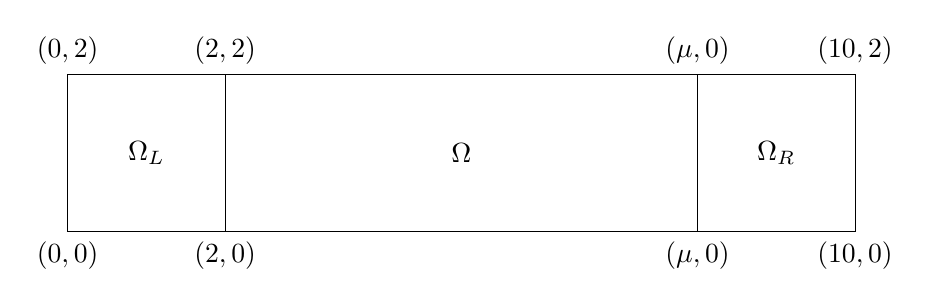
\begin{tikzpicture}
\draw (0,0) node[anchor=north]{$(0,0)$}
  -- (2,0) node[anchor=north]{$(2,0)$}
  -- (2,2) node[anchor=south]{$(2,2)$}
  -- (0,2) node[anchor=south]{$(0,2)$}
  -- cycle;
\node at (1,1){$\Omega_L$};
\draw (2,0) node[anchor=north]{}
  -- (8,0) node[anchor=north]{}
  -- (8,2) node[anchor=south]{}
  -- (2,2) node[anchor=south]{}
  -- cycle;
\node at (5,1){$\Omega$};
\draw (8,0) node[anchor=north]{$(\mu,0)$}
  -- (10,0) node[anchor=north]{$(10,0)$}
  -- (10,2) node[anchor=south]{$(10,2)$}
  -- (8,2) node[anchor=south]{$(\mu,0)$}
  -- cycle;
\node at (9,1){$\Omega_R$};
\end{tikzpicture}
\captionof{figure}{Parametrized domain} 
\label{parametrized_domain}
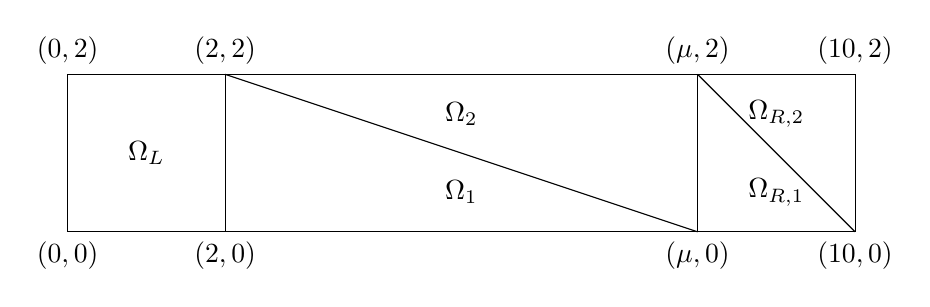
\begin{tikzpicture}
\draw (0,0) node[anchor=north]{$(0,0)$}
  -- (2,0) node[anchor=north]{$(2,0)$}
  -- (2,2) node[anchor=south]{$(2,2)$}
  -- (0,2) node[anchor=south]{$(0,2)$}
  -- cycle;
\node at (1,1){$\Omega_L$};
\draw (2,0) node[anchor=north]{}
  -- (8,0) node[anchor=north]{}
  -- (8,2) node[anchor=south]{}
  -- (2,2) node[anchor=south]{}
  -- cycle;
\node at (5,0.5){$\Omega_1$};
\node at (5,1.5){$\Omega_2$};
\draw (2,2) node[anchor=north]{}
  -- (8,0) node[anchor=north]{}
  -- cycle;
\draw (8,0) node[anchor=north]{$(\mu,0)$}
  -- (10,0) node[anchor=north]{$(10,0)$}
  -- (10,2) node[anchor=south]{$(10,2)$}
  -- (8,2) node[anchor=south]{$(\mu,2)$}
  -- cycle;
\draw (8,2) node[anchor=north]{}
  -- (10,0) node[anchor=north]{}
  -- cycle;
\node at (9,0.5){$\Omega_{R,1}$};
\node at (9,1.5){$\Omega_{R,2}$};
\end{tikzpicture}
\captionof{figure}{Parametrized domain divided into subdomains} 
\label{parametrized_domain_subdomains}
\end{figure}

We further divide $\Omega$ into triangular subdomains $\Omega_1,\Omega_2$ i.e. $\Omega = \Omega_1 \cup \Omega_2$ and divide $\Omega_R$ into triangular subdomains $\Omega_{R,1},\Omega_{R,2}$ i.e. $\Omega_R = \Omega_{R,1} \cup \Omega_{R,2}$ (Figure \ref{parametrized_domain_subdomains}). The division into triangular subdomain makes the mapping between reference domain and parametrized domain affine.

We consider the parameter variation within range $\mu = [7,9]$. We refer to $\hat{\Omega}_1$ and $\hat{\Omega}_2$ as the domain at reference parameter $\tilde{\mu}$. The parametric mappings are
\begin{equation}
\begin{split}
F_1 : \hat{\Omega}_1 \times \mathbb{P} \rightarrow \Omega_1 \ , \
T_1 : \Omega_1 \times \mathbb{P} \rightarrow \hat{\Omega}_1 \ , \\
F_2 : \hat{\Omega}_2 \times \mathbb{P} \rightarrow \Omega_2 \ , \
T_2 : \Omega_2 \times \mathbb{P} \rightarrow \hat{\Omega}_2 \ , \\
F_{R,1} : \hat{\Omega}_{R,1} \times \mathbb{P} \rightarrow \Omega_{R,1} \ , \
T_{R,1} : \Omega_{R,1} \times \mathbb{P} \rightarrow \hat{\Omega}_{R,1} \ ; \\
F_{R,2} : \hat{\Omega}_{R,2} \times \mathbb{P} \rightarrow \Omega_{R,2} \ , \
T_{R,2} : \Omega_{R,2} \times \mathbb{P} \rightarrow \hat{\Omega}_{R,2} \ .
\end{split}
\end{equation}
where, 
\begin{equation}
\begin{split}
x = F_n(\hat{x},\mu) = (G_F)_n(\mu) \hat{x} + (c_F)_n(\mu) \ , \\
\hat{x} = T_n(x,\mu) = (G_T)_n(\mu) x + (c_T)_n(\mu) \ ,\\
x \in \Omega_n, \hat{x} \in \hat{\Omega}_n \ , \ n = 1,2 \ ,
\end{split}
\end{equation}
and
\begin{equation}
\begin{split}
x = F_n(\hat{x},\mu) = (G_F)_{R,n}(\mu) \hat{x} + (c_F)_{R,n}(\mu) \ , \\
\hat{x} = T_n(x,\mu) = (G_T)_{R,n}(\mu) x + (c_T)_{R,n}(\mu) \ , \\
x \in \Omega_{R,n}, \hat{x} \in \hat{\Omega}_{R,n} \ , \ n = 1,2 \ .
\end{split}
\end{equation}

The Jacobians can be computed as,

\begin{equation}\label{transformation_matrices_subsdomain}
\begin{split}
(G_F)_1 =
\begin{spmatrix}{}
    \frac{2-\mu}{2-\tilde{\mu}} & 0 \\
    0 & 1
\end{spmatrix}
\ , \
(G_T)_1 =
\begin{spmatrix}{}
    \frac{2-\tilde{\mu}}{2-\mu} & 0 \\
    0 & 1
\end{spmatrix}
\ ; \\
(G_F)_2 =
\begin{spmatrix}{}
    \frac{2-\mu}{2-\tilde{\mu}} & 0 \\
    0 & 1
\end{spmatrix}
\ , \
(G_T)_2 =
\begin{spmatrix}{}
    \frac{2-\tilde{\mu}}{2-\mu} & 0 \\
    0 & 1
\end{spmatrix}
\ ; \\
(G_F)_{R,1} =
\begin{spmatrix}{}
    \frac{10 - \mu}{10 - \tilde{\mu}} & 0 \\
    0 & 1
\end{spmatrix}
\ , \
(G_T)_{R,1} =
\begin{spmatrix}{}
    \frac{10 - \tilde{\mu}}{10 - \mu} & 0 \\
    0 & 1
\end{spmatrix}
\ ; \\
(G_F)_{R,2} =
\begin{spmatrix}{}
    \frac{10 - \mu}{10 - \tilde{\mu}} & 0 \\
    0 & 1
\end{spmatrix}
\ , \
(G_T)_{R,2} =
\begin{spmatrix}{}
    \frac{10 - \tilde{\mu}}{10 - \mu} & 0 \\
    0 & 1
\end{spmatrix}
\ .
\end{split}
\end{equation}

By substituting the equation \eqref{transformation_matrices_subsdomain} in the equations \eqref{affine_diffusive_term} - \eqref{affine_source_term}, we get,

\begin{equation}
\begin{split}
(\nu \frac{\partial \phi_i}{\partial x_k} , \frac{\partial \phi_j}{\partial x_k})_{\Omega_1} = \left(\frac{2 - \tilde{\mu}}{2 - \mu} \right) \int_{\hat{\Omega}_1} \nu \frac{\partial \hat{\phi}_i}{\partial \hat{x}_1} \cdot \frac{\partial \hat{\phi}_j}{\partial \hat{x}_1} + 0 \int_{\hat{\Omega}_1} \nu \frac{\partial \hat{\phi}_i}{\partial \hat{x}_1} \cdot \frac{\partial \hat{\phi}_j}{\partial \hat{x}_2} \\ + 0 \int_{\hat{\Omega}_1} \nu \frac{\partial \hat{\phi}_i}{\partial \hat{x}_2} \cdot \frac{\partial \hat{\phi}_i}{\partial \hat{x}_1} + \left( \frac{2 - \mu}{2 - \tilde{\mu}} \right) \int_{\hat{\Omega}_1} \nu \frac{\partial \hat{\phi}_j}{\partial \hat{x}_2} \cdot \frac{\partial \hat{\phi}_j}{\partial \hat{x}_2} \ .
\end{split}
\end{equation}

The expression under integral on $\Omega_1$ is not evaluated repeatedly and evaluated only over the domain $\hat{\Omega}_1$. The number of $FLOPS$ for evaluating integral by $n-$point quadrature rule is $n(n-1)$ (not considering the $FLOPS$ for evaluating the function under integral). In return, a simplified expression dependent only on parameter $\mu$ is required to be evaluated. The number of these expressions is number of parameter dependent subdomains i.e. $4$, in this case. Hence, by avoiding the expensive operation of evaluating the integral, significant time saving is achieved. 

\chapter{Reduced basis method}

\section{Snapshot proper orthogonal decomposition}\label{POD_section}

We present now snapshot proper orthogonal decomposition method. Here, ``snapshot" means solution calculated by discontinuous Galerkin method. We calculate solution based on $\mu_n, n \in \lbrace 1,....,n_s \rbrace$ i.e. $n_s$ snapshots are generated. We also introduce inner product matrices $M_u \in \mathbb{R}^{u_{ndofs} \times u_{ndofs}}$ and $M_p \in \mathbb{R}^{p_{ndofs} \times p_{ndofs}}$, formed by inner product of basis function with respect to suitable function space $\mathbb{W}$.

\begin{equation}
M_u = <\phi,\phi>_{\mathbb{W}} \ .
\end{equation}

\begin{equation}
M_p = <\psi,\psi>_{\mathbb{W}} \ .
\end{equation}

We also introduce matrices storing velocity snapshots $S_u$ and storing pressure snapshots $S_p$. We discuss the method only for velocity snapshots. The method is similar for pressure snapshots. We note the size of matrices, useful for matrix operations presented hereafter.

\begin{center}

$S_u \in \mathbb{R}^{u_{ndofs} \times n_s} \ ,$\\
$S_p \in \mathbb{R}^{p_{ndofs} \times n_s} \ ,$\\
$M_u \in \mathbb{R}^{u_{ndofs} \times u_{ndofs}} \ ,$\\
$M_p \in \mathbb{R}^{p_{ndofs} \times p_{ndofs}} \ .$\\

\end{center}

\subsection{Spectral decomposition of snapshots}

We denote the dimension of reduced basis as $N$ and assert that $N < n_s$. We now perform the spectral decomposition of $S_u^TM_uS_u$,

\begin{equation}
S_u^TM_uS_u = V \Theta V^T \textrm{.}
\end{equation}

The columns of $V$ are eigenvectors and $\Theta$ has eigenvalues $\theta$ such that,

\begin{equation}
\Theta_{ij} = \theta_{ij} \delta_{ij} \textrm{.}
\end{equation}

We also note that $\theta_{ij} > 0$ and $\theta_1 \geq \theta_2 \geq ... \geq \theta_{n_s}$ i.e. the eigenvalues are in sorted order. We form the reduced basis by linear combination of the snapshot vector,
\begin{equation}
B_{velocity} = S_u A \textrm{,} \quad A \in \mathbb{R}^{n_s \times N} \textrm{.}
\end{equation}

Here,$B_{velocity}$ is defined such that, if $\phi \in \mathbb{R}^{n \times d_u}$ $B_{velocity} \in \mathbb{R}^{n \times N}$, the reduced basis for velocity $\psi_u \in \mathbb{R}^{d_u \times N}$ is formed by,
\begin{equation}
\psi_u = \phi^T B \textrm{.}
\end{equation}

Considering orthonormality of reduced basis $\psi_u$ with respect to inner product in function space $\mathbb{W}$,

\begin{equation}
<\psi_u , \psi_u>_{\mathbb{W}} = B_u^T M_{u} B_u = I \ .
\end{equation}

Considering above orthonormality, we express matrix $A$ as,
\begin{equation}
A = V \Theta^{-\frac{1}{2}} R \textrm{,} \quad R \in \mathbb{R}^{n_s \times N} \textrm{,} \quad R^TR = I \textrm{.}
\end{equation}

where, $I$ is identity matrix of suitable size.

We set now $R$ as,
\begin{equation}
R = [I_{N \times N} ; 0_{(n_s \times N)}] \quad \textrm{ and accordingly} \quad B = S V \Theta^{-\frac{1}{2}} R \textrm{.}
\end{equation}

\section{Galerkin reduced basis formulation}\label{Galerkin_section}

We now present the reduced bilinear form as,

\begin{equation} \label{stokes_equation_parameter}
a(u_N,\phi_N;\mu) + b(p_N,\phi_N;\mu) = f_1(\phi_N,\mu) \textrm{,}
\end{equation}

\begin{equation} \label{continuity_equation_parameter}
b(u_N,\psi_N;\mu) = f_2(\psi_N,\mu) \textrm{.}
\end{equation}

In discrete form, we form reduced equation as,

\begin{equation} \label{Stokes_matrix_reduced}
\begin{spmatrix}{\tilde{K}}
    B_{velocity}^T A(\mu) B_{velocity} & B_{velocity}^T B(\mu) B_{pressure} \\
    B_{pressure}^T B(\mu)^T B_{velocity} & 0
\end{spmatrix}
\begin{spmatrix}{\zeta}
    U_N \\
    P_N
\end{spmatrix}
=
\begin{spmatrix}{\tilde{F}}
    B_{velocity}^T F_1(\mu)  \\
    B_{pressure}^T F_2(\mu)
\end{spmatrix} \textrm{,}
\end{equation}

and accordingly we solve following variational form for reduced degrees of freedom $\zeta$,
\begin{equation}
\tilde{K} \zeta = \tilde{F} \textrm{,} \quad \zeta_u \in \mathbb{R}^{N} \textrm{,}
\end{equation}

and calculate reduced solution $u_N$ as,
\begin{equation}
u_N = \psi_u \zeta_u \textrm{,} \quad u_N \in \mathbb{R}^{d_u} \textrm{.}
\end{equation}

\chapter{Numerical example}

\section{Lid-driven cavity problem} \label{lid_driven_cavity_stokes}

We next present a benchmark $CFD$ problem, the Lid-driven cavity flow \cite{Montlaur2}. We solve the Stokes flow on the unit square [0,1] $\times$ [0,1] in the $x-y$ plane. On boundaries ${x = 0}, {x = 1}$ and ${y = 0}$, we impose no slip or zero velocity Dirichlet condition. On ${y = 1}$, we impose Dirichlet condition with Dirichlet velocity,
\begin{equation}
\begin{split}
u = (10x,0) \quad \textrm{for} \quad 0 \leq x \leq 0.1 \textrm{,}\\
u = (1,0) \quad \textrm{for} \quad 0.1 \leq x \leq 0.9 \textrm{,}\\
u = (10 - 10x,0) \quad \textrm{for} \quad 0.9 \leq x \leq 1 \textrm{.}
\end{split}
\end{equation}

The results are shown in Figure \ref{stoke_schur_lid}. The results are found to be in agreement with literature i.e. boundary layer formation at the no slip boundaries and shape of streamline. 

\begin{figure}
\begin{subfigure}{\textwidth}	
  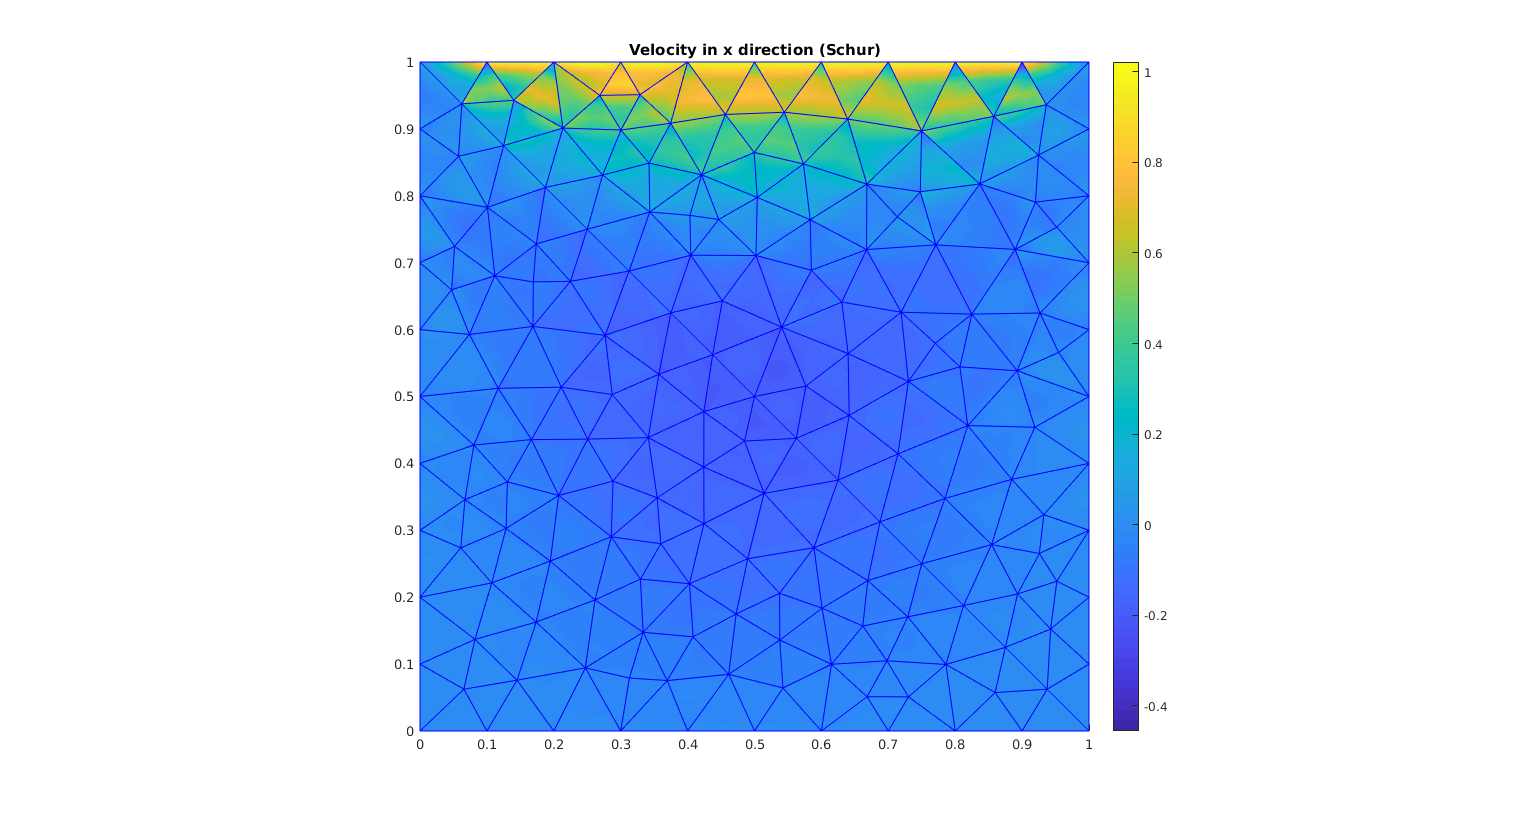
\includegraphics[width=0.8\linewidth]{velocity_x_lid_driven_cavity.png}
  \caption{$x-$velocity} 
  \label{x_vel_stoke_schur_lid}
\end{subfigure}
\begin{subfigure}{\textwidth}	
  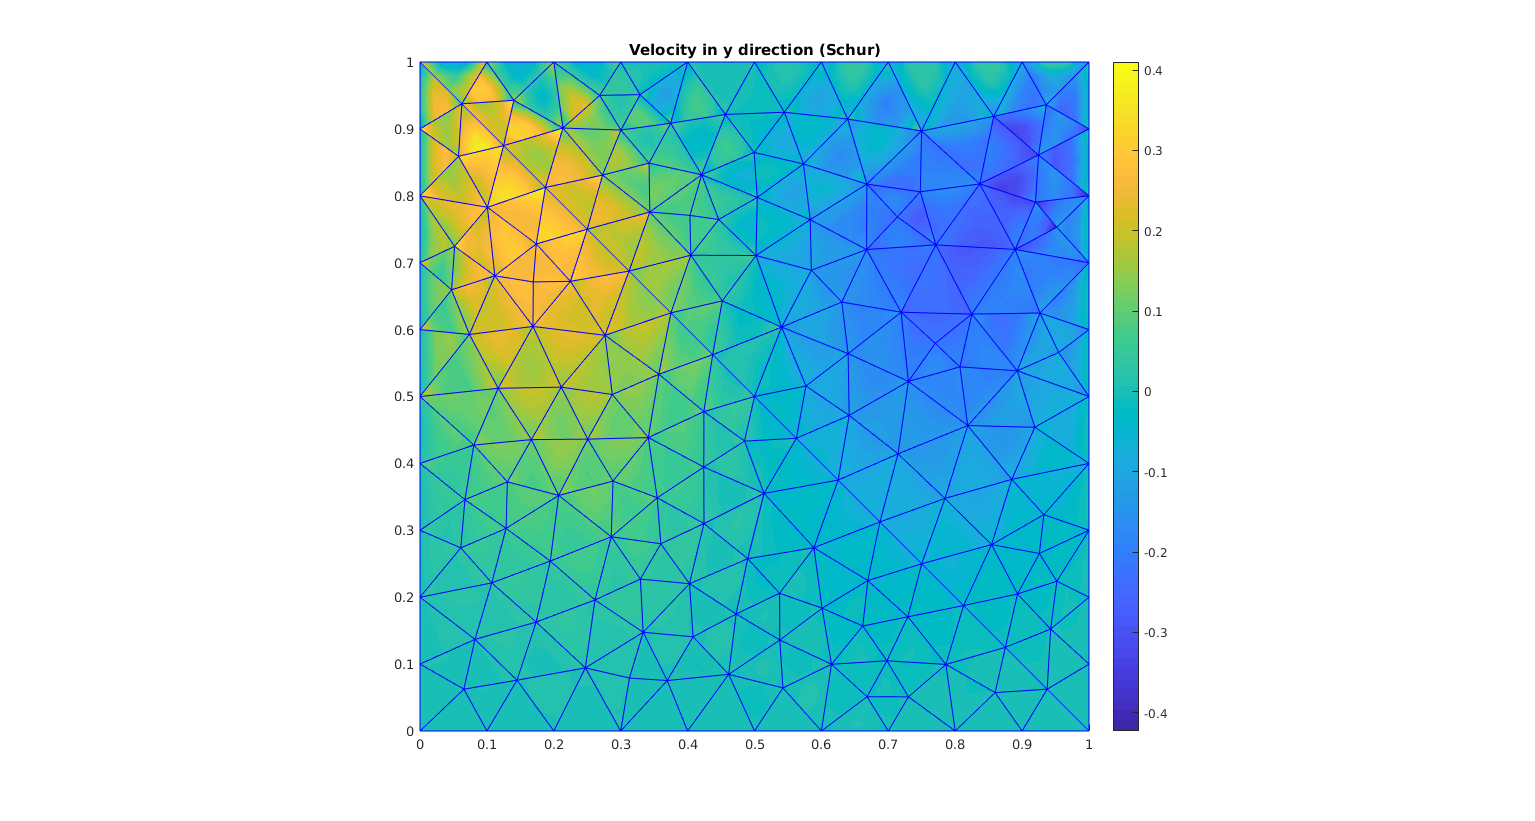
\includegraphics[width=0.8\linewidth]{velocity_y_lid_driven_cavity.png}
    \caption{$y-$velocity} 
    \label{y_vel_stoke_schur_lid}
\end{subfigure}
\begin{subfigure}{\textwidth}	
  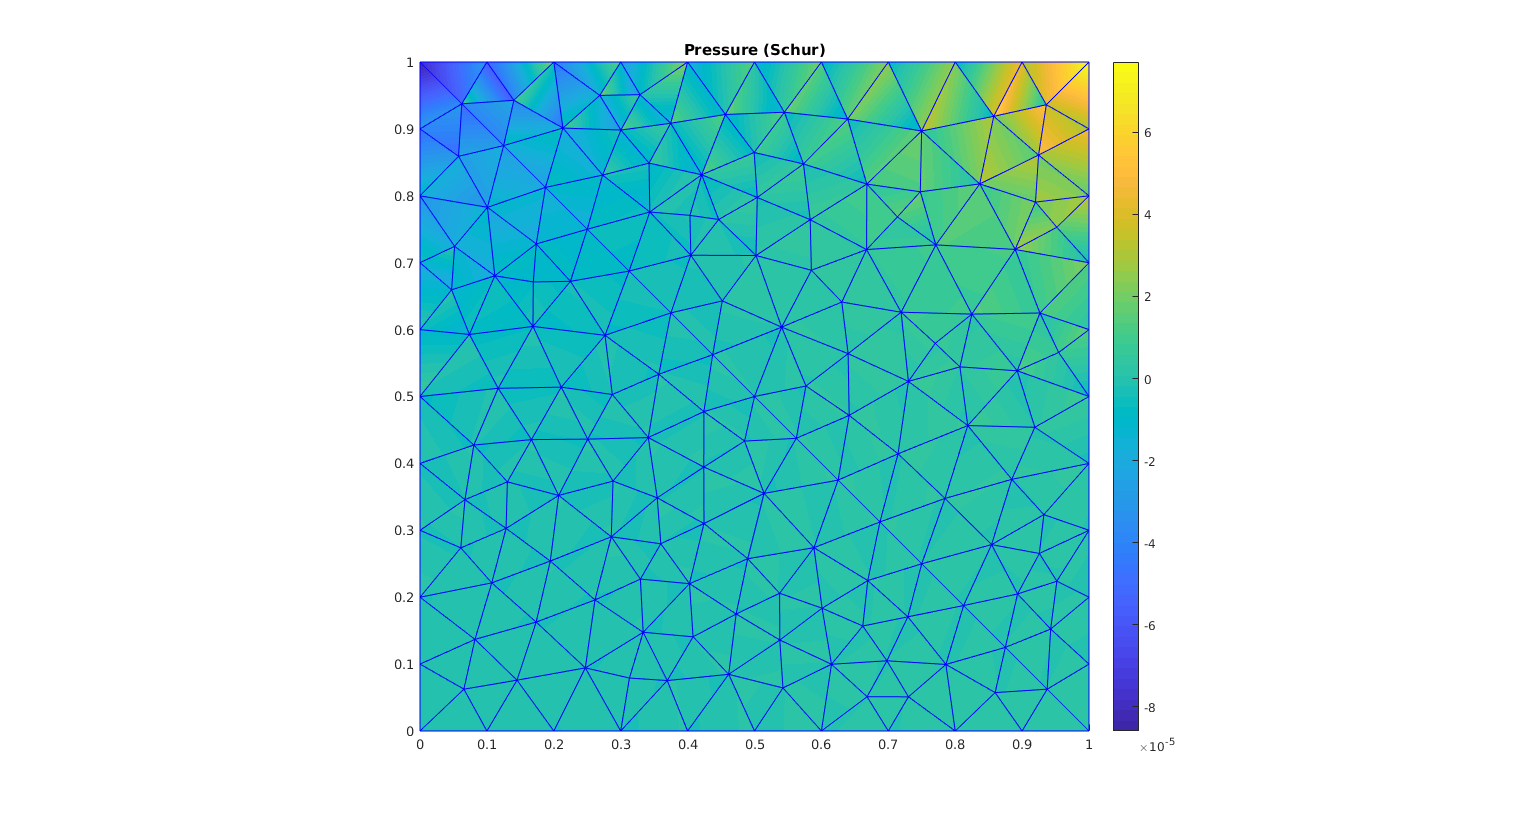
\includegraphics[width=0.8\linewidth]{pressure_lid_driven_cavity.png}
    \caption{Pressure} 
    \label{pressure_stoke_schur_lid}
\end{subfigure}
\caption{Lid driven cavity problem (Schur complement method)}
\label{stoke_schur_lid}
\end{figure}

\section{Analytical example}

The domain considered for this example is the unit square [0,1] $\times$ [0,1] in the $x-y$ plane. 
The boundary ${x=0}$ is dirichlet boundary with inflow velocity at point $(0,y)$ as $u = (y(1-y), 0)$. The boundaries ${y = 0}$ and ${y = 1}$ are Dirichlet boundaries with no slip or zero velocity condition. The boundary ${x = 1}$ is a Neumann boundary with zero Neumann value i.e. $t = (0, 0)$. The source term is $f = (2 \nu - 1, 0)$. The analytical solution for pressure and velocity reads as,

\begin{center}

\begin{equation}
p = (1 - x) \textrm{,}
\end{equation}

\begin{equation} 
 u = (y(1-y), 0) \textrm{.}
\end{equation}

\end{center}

The results of an $h-$convergence test with velocity polynomial degree $D=2$ and pressure polynomial degree $D-1 = 2$ in the $L^2$ norm is presented in Figures \ref{convergence_check_velocity} and \ref{convergence_check_pressure}.

\begin{figure}
\begin{subfigure}{\textwidth}	
  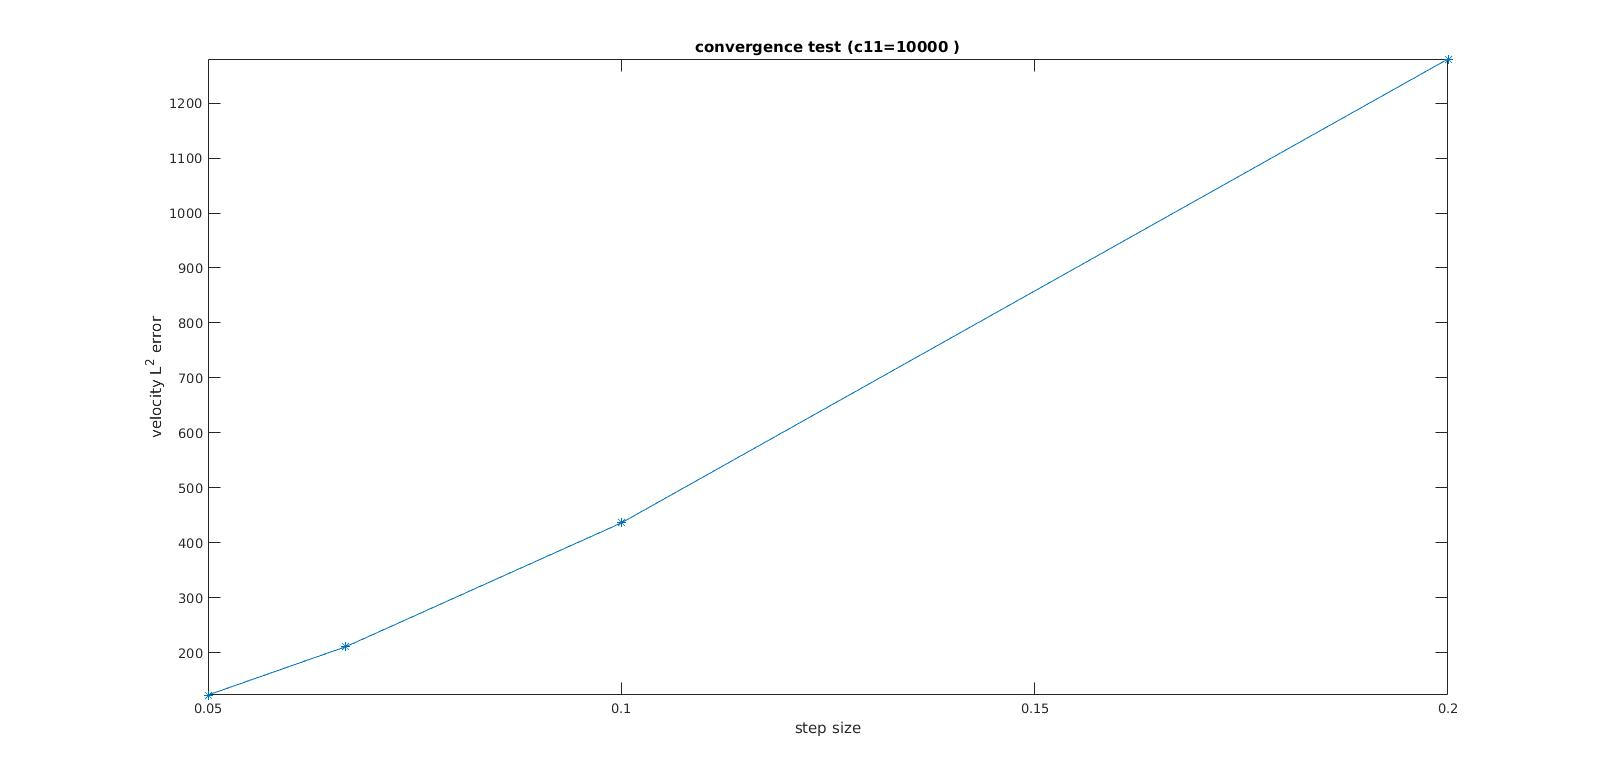
\includegraphics[width=\linewidth]{step_size_vs_velocity_l2_error.jpg}
  \caption{step size vs $L^2$ error in velocity} 
  \label{step_size_vs_velocity_l2_error}
  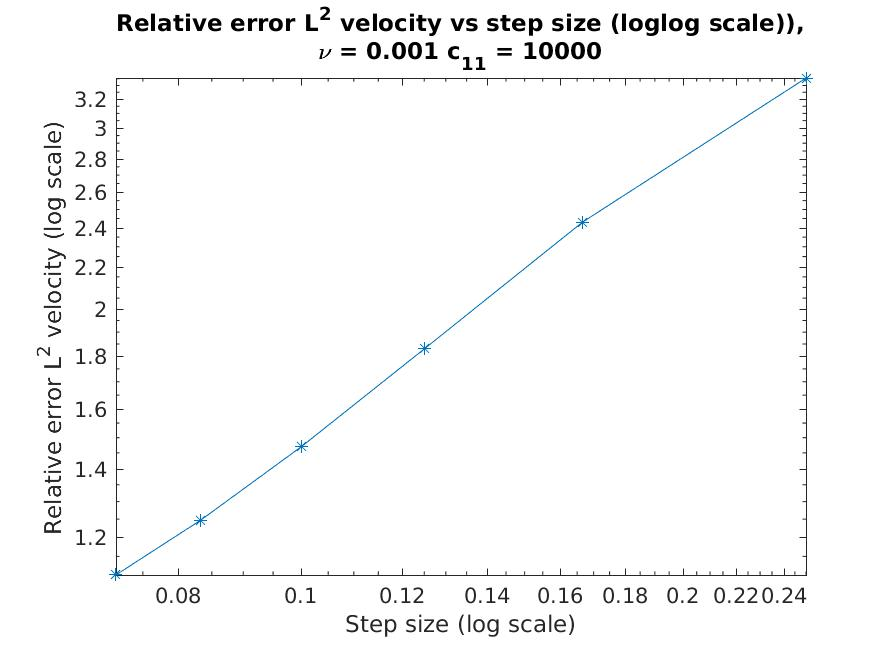
\includegraphics[width=\linewidth]{step_size_vs_velocity_l2_error_loglog.jpg}
  \caption{step size vs $L^2$ error in velocity (loglog scale)} 
  \label{step_size_vs_velocity_l2_error_loglog}
\end{subfigure}
\caption{Convergence test for velocity}
\label{convergence_check_velocity}
\end{figure}

\begin{figure}
\begin{subfigure}{\textwidth}	
  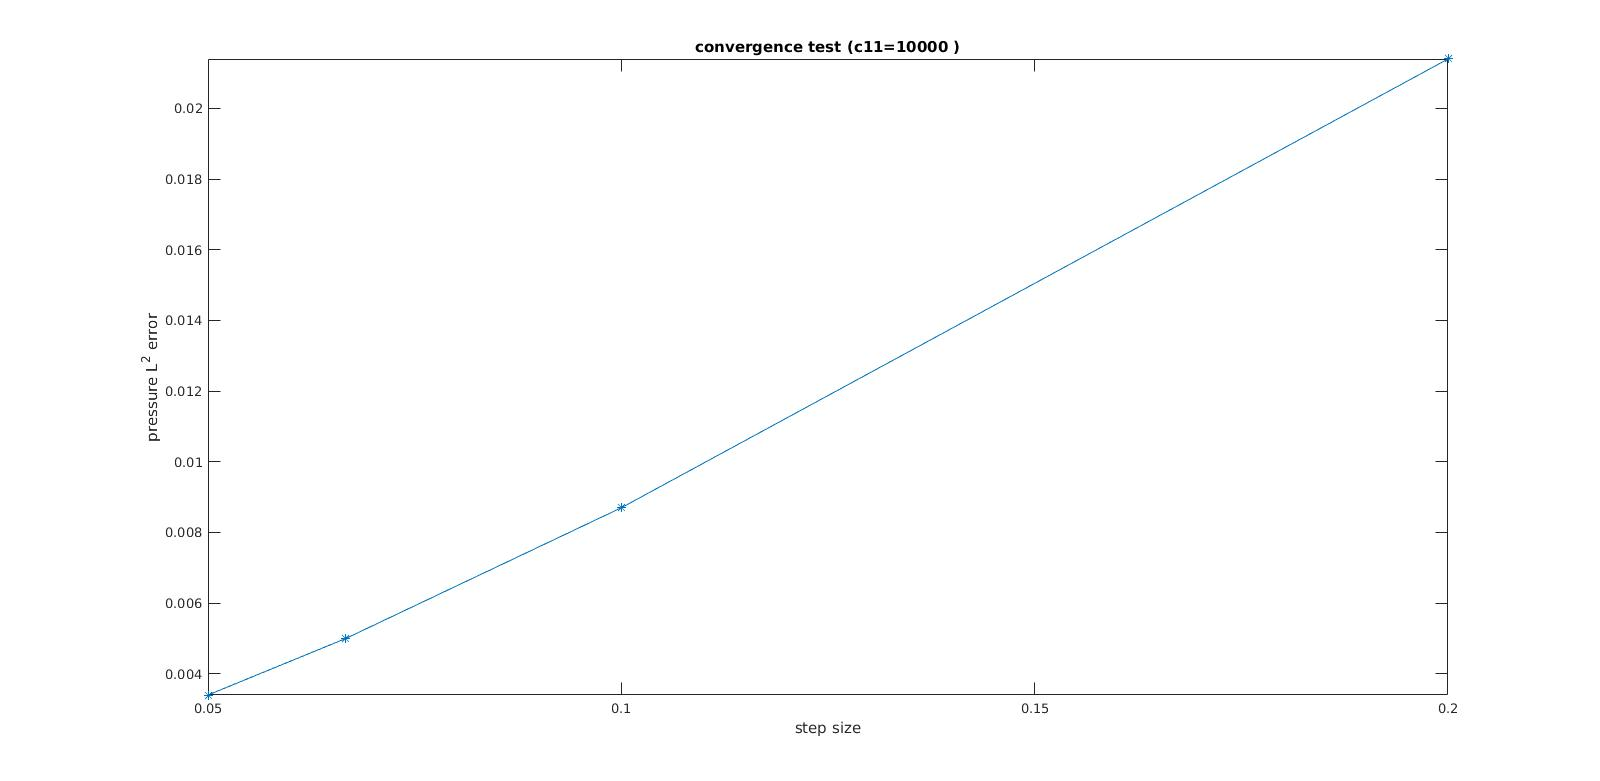
\includegraphics[width=\linewidth]{step_size_vs_pressure_l2_error.jpg}
  \caption{step size vs $L^2$ error in pressure} 
  \label{step_size_vs_pressure_l2_error}
  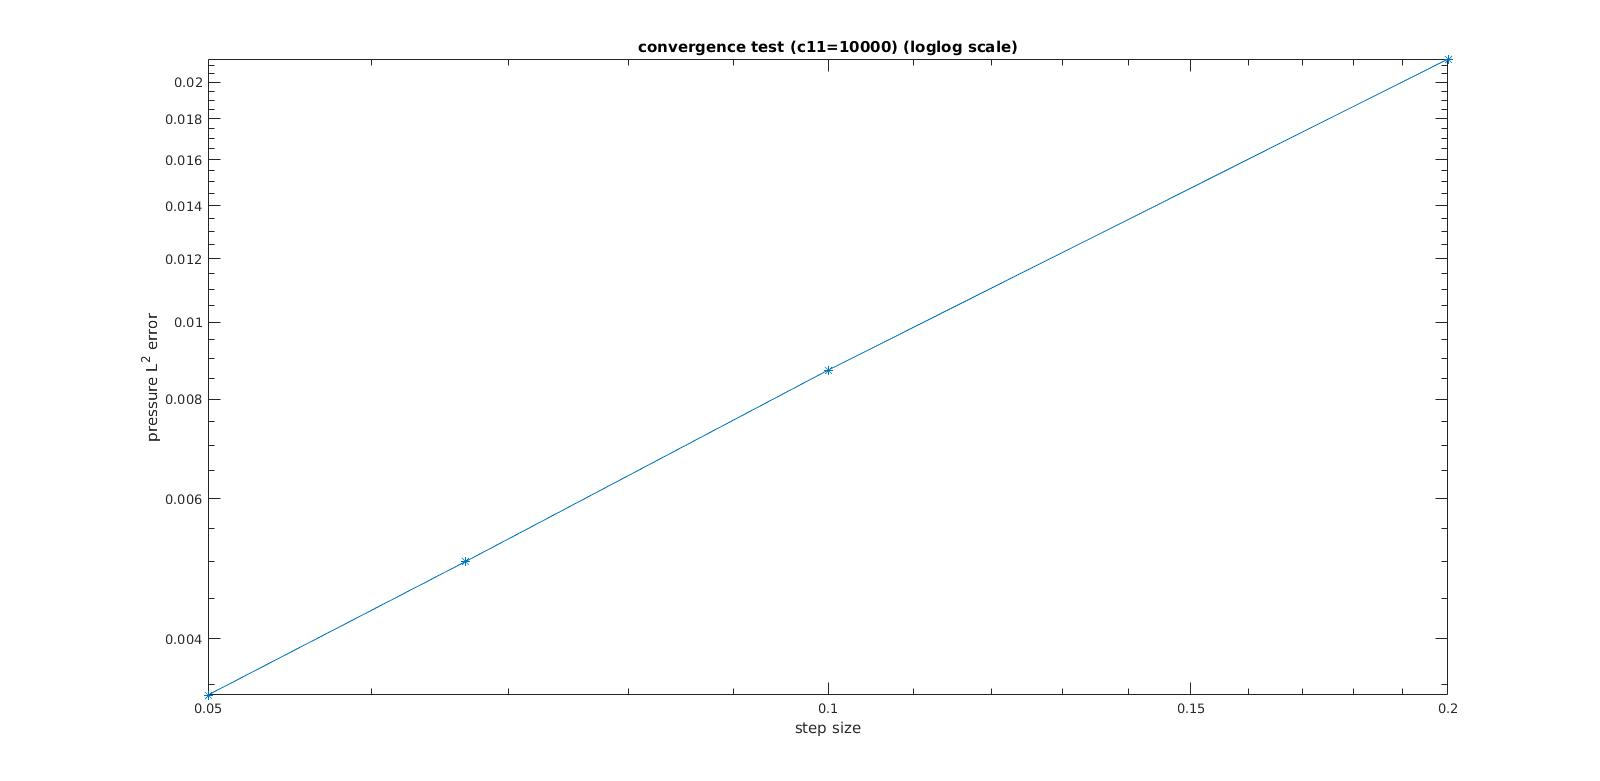
\includegraphics[width=\linewidth]{step_size_vs_pressure_l2_error_loglog.jpg}
  \caption{step size vs $L^2$ error in pressure (loglog scale)} 
  \label{step_size_vs_pressure_l2_error_loglog}
\end{subfigure}
\caption{Convergence test for pressure}
\label{convergence_check_pressure}
\end{figure}

Additionally, we also compare the impact of changing coercivity parameter $c11$ on condition number and error in the solution (Figure \ref{all_c11_figure}, \ref{all_c11_figure_semilog}). The number of divisions in each direction is 10. The lowest value of $c11$ considered is the value that is required to maintain coercivity.

\begin{figure}
\begin{subfigure}{\textwidth}	
  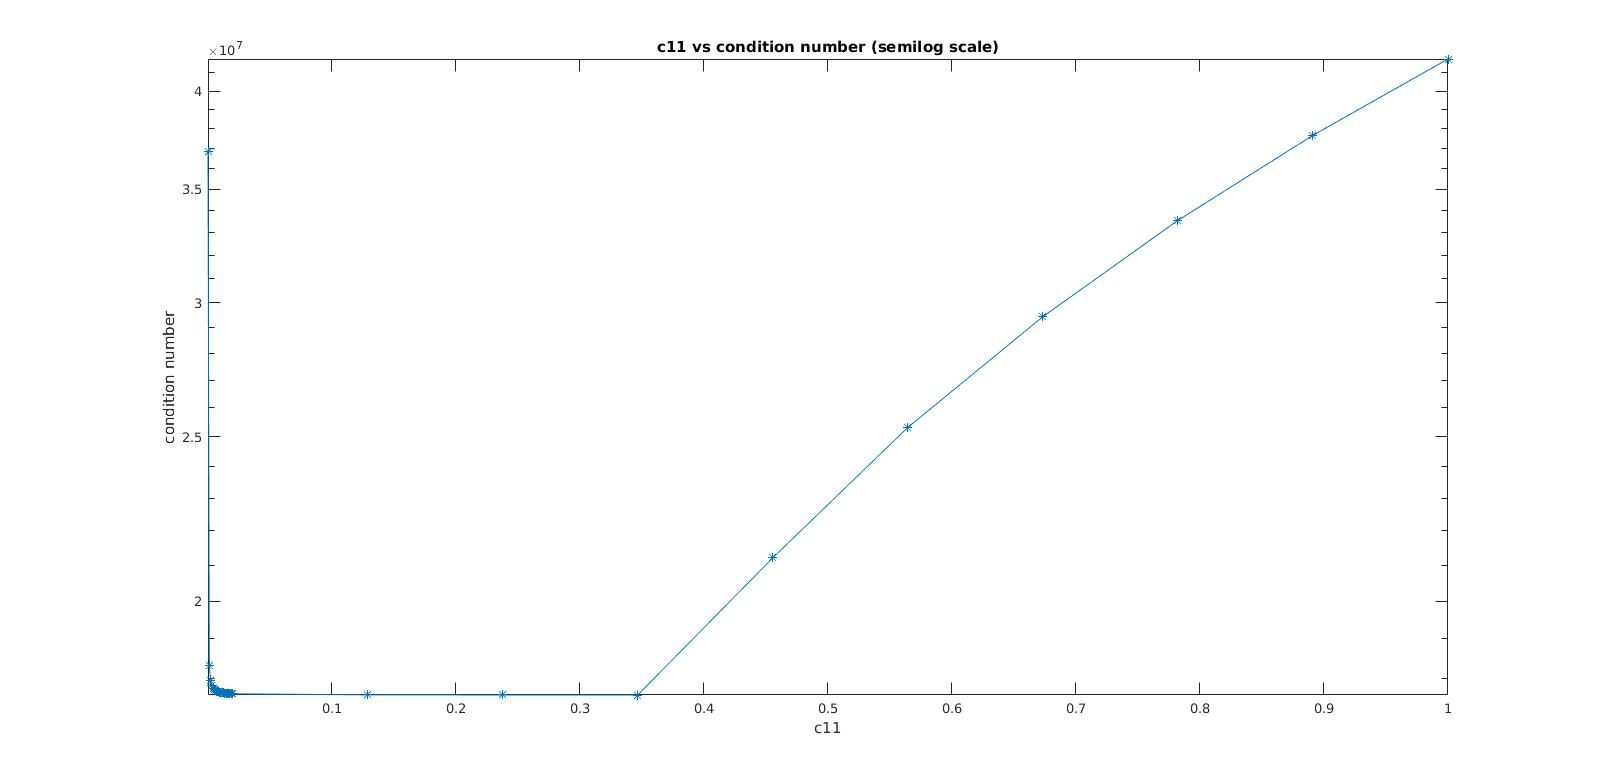
\includegraphics[width=0.8\linewidth]{c11_condition_number_semilog.jpg}
  \caption{$c11$ vs condition number (semilog scale)} 
  \label{$c11$ vs Condition number_semilog}
  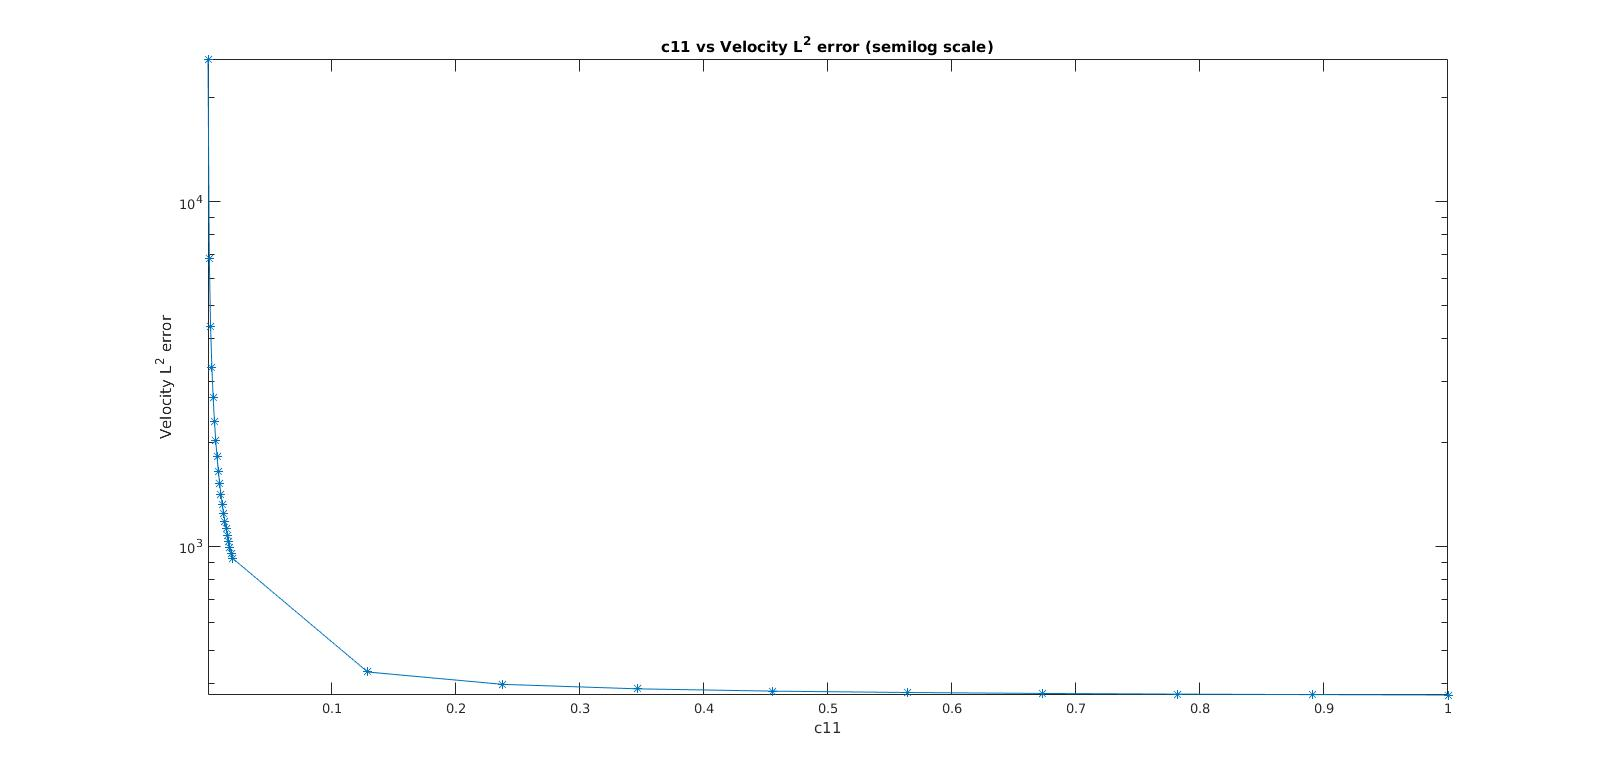
\includegraphics[width=0.8\linewidth]{c11_velocity_l2_error_semilog.jpg}
  \caption{$c11$ vs $L^2$ error in velocity (semilog scale)} 
  \label{c11_L2_error_velocity_semilog}
  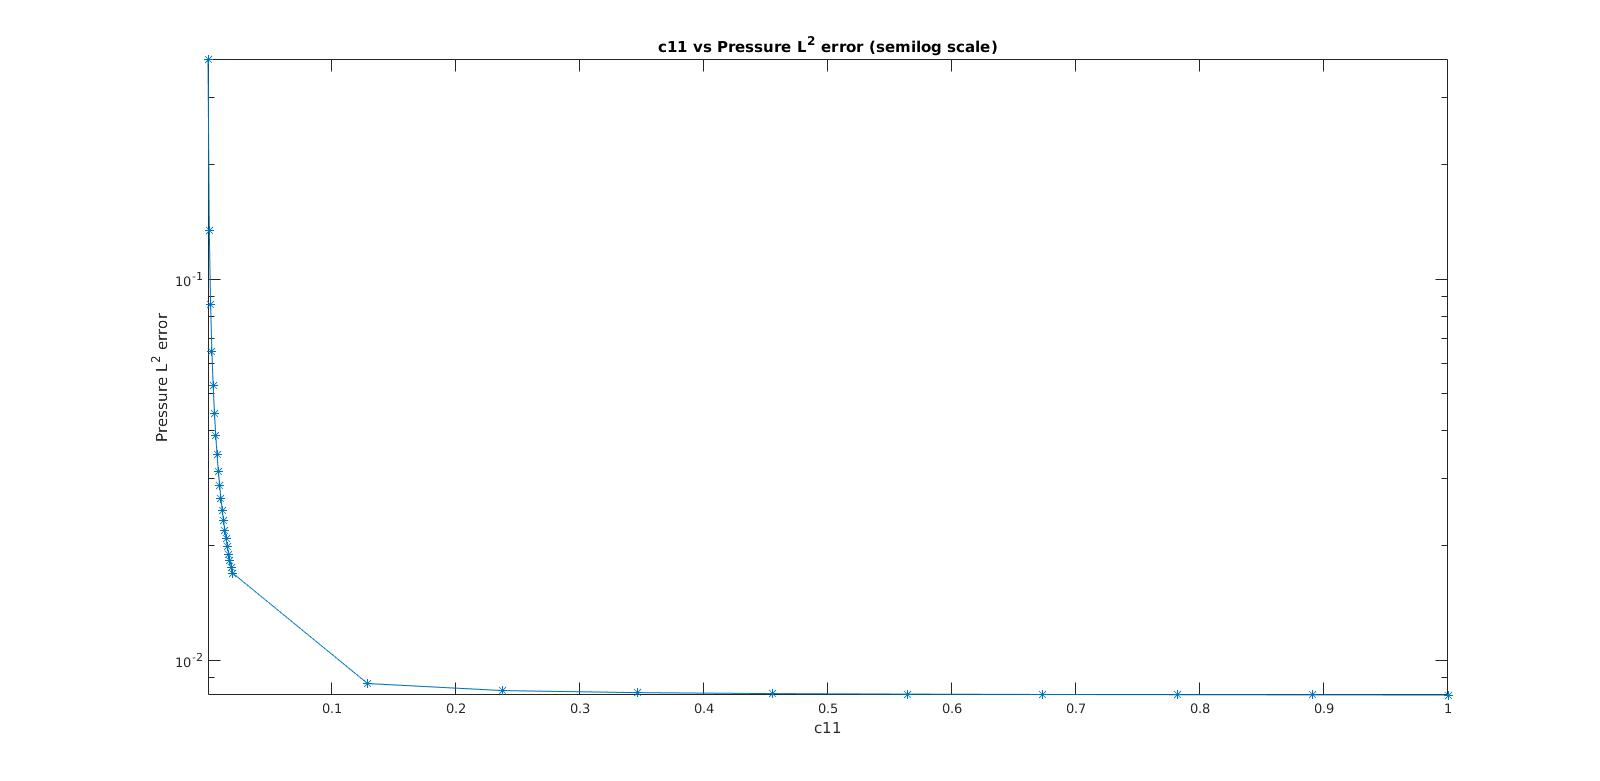
\includegraphics[width=0.8\linewidth]{c11_pressure_l2_error_semilog.jpg}
  \caption{$c11$ vs $L^2$ error in pressure (semilog scale)} 
  \label{c11_L2_error_pressure_semilog}
\end{subfigure}
\caption{Impact of $c11$ on condition number, velocity and pressure $L^2$ error (loglog scale)}
\label{all_c11_figure_semilog}
\end{figure}

\section{POD-Galerkin method}

We perform the POD-Galerkin method as mentioned in section \ref{POD_section} and section \ref{Galerkin_section}. The boundary ${x=0}$ is dirichlet boundary with inflow velocity at point $(0,y)$ as $u = (y(1-y), 0)$. The boundary ${x = 1}$ is a Neumann boundary with zero Neumann value i.e. $t = (0, 0)$. Other boundaries are Dirichlet boundary with no slip condition. The source term is $f = (2 \nu - 1, 0)$. We consider inner-product matrix as Discontinuous Galerkin mass matrix i.e.
\begin{gather}
M_u = \int_{\Omega} \phi_i \phi_j \ , \ i,j = 1, \ldots, u_{ndofs} \ . \\
M_p = \int_{\Omega} \psi_i \psi_j \ , \ i,j = 1, \ldots, p_{ndofs} \ .
\end{gather}

The domain is shown in Figure \ref{pod_figure}. The geometric parameters were coordinates of tip of the obstacle.
\begin{gather}
(x,y) = (\mu_1,\mu_2) \ . \\
(x_{ref},y_{ref}) = (0.5,0.3) \ .
\end{gather}

We show eigenvalue decay of the snapshot matrix (Figure \ref{pod_eigenvalue_figure}, \ref{pod_eigenvalue_figure_semilog}). The parameters for generating snapshots were generated randomly over space $[0.4,0.6] \times [0.2,0.4]$. The number of parameters considered were $40$. 

The reduced basis error was measured at $10$ random points in parameter space (Figure \ref{rb_error}).

\begin{figure}
  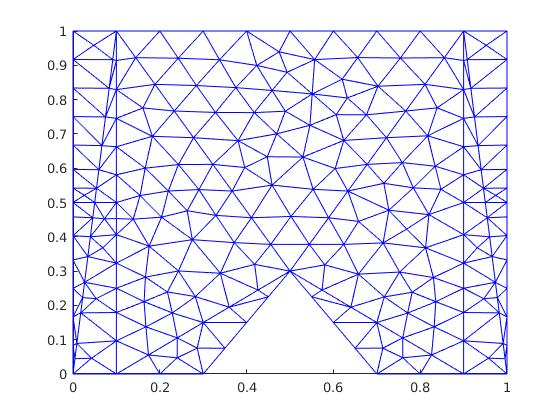
\includegraphics[width=\linewidth]{pod_figure.jpg}
  \caption{Domain $\Omega$} 
  \label{pod_figure}
\end{figure}

\begin{figure}
\begin{subfigure}{\textwidth}	
  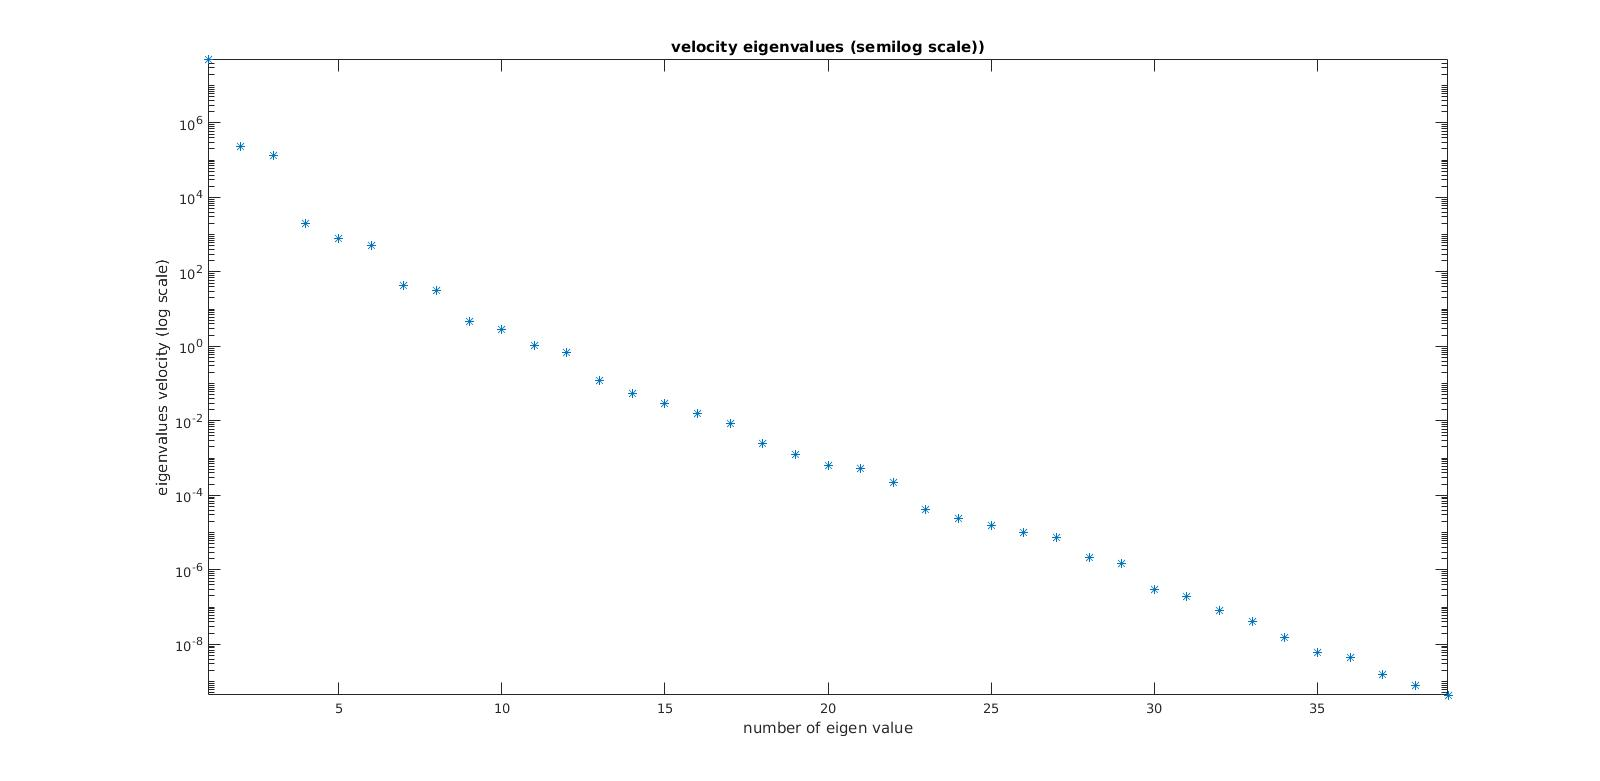
\includegraphics[width=\linewidth]{velocity_eigen_value_semilog.jpg}
  \caption{Velocity Eigenvalue decay (semilog scale)} 
  \label{eigen_value_decay_velocity_semilog}
  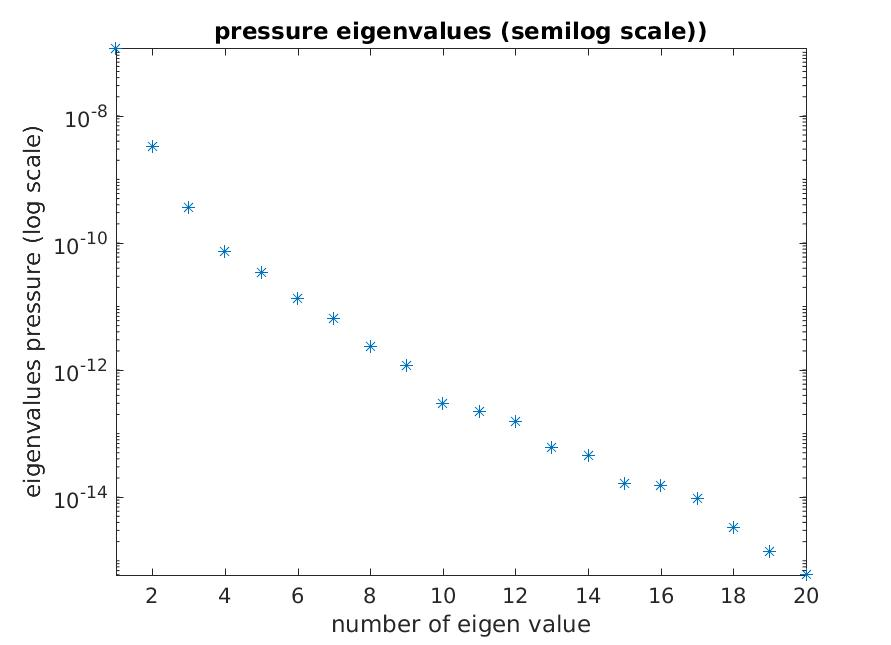
\includegraphics[width=\linewidth]{pressure_eigen_value_semilog.jpg}
  \caption{Pressure Eigenvalue decay (semilog scale)} 
  \label{eigen_value_decay_pressure_semilog}
\end{subfigure}
\caption{Eigenvalue decay for velocity and pressure}
\label{pod_eigenvalue_figure_semilog}
\end{figure}

\begin{figure}
\begin{subfigure}{\textwidth}	
  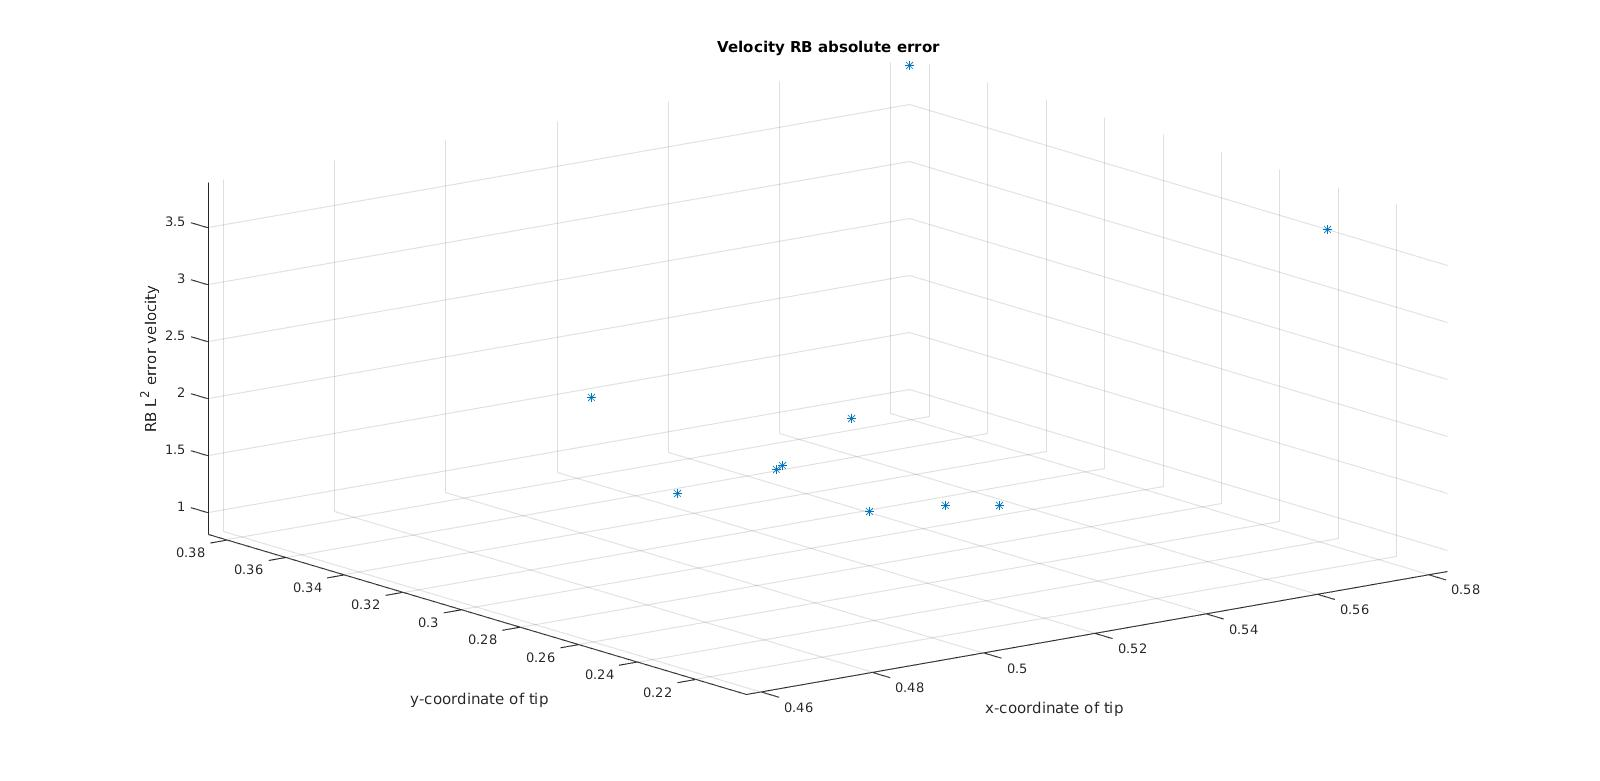
\includegraphics[width=\linewidth]{rb_l2_error_velocity.jpg}
  \caption{Reduced basis $L^2$ error for velocity} 
  \label{rb_L2_error_velocity}
  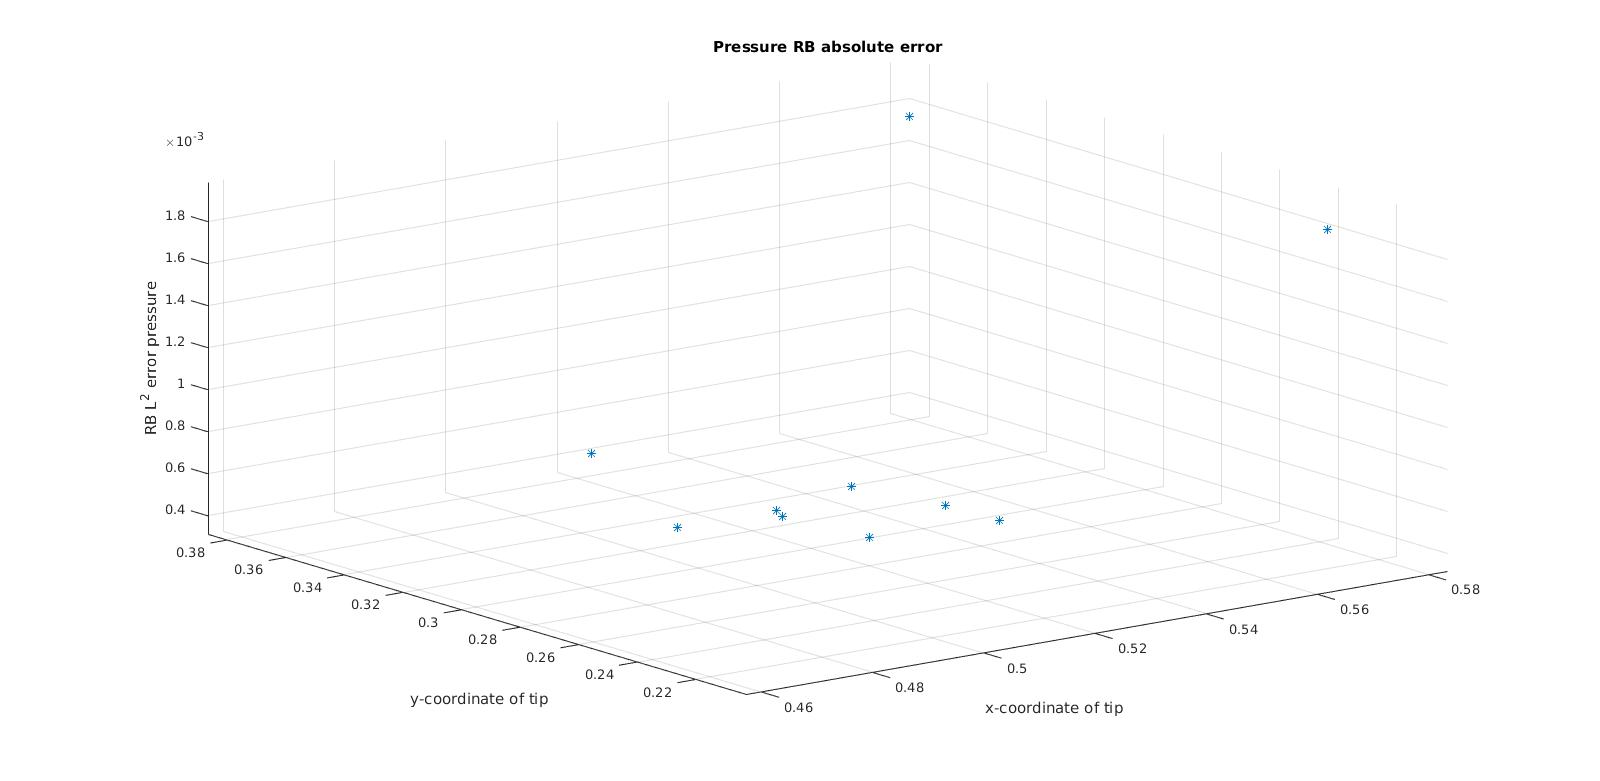
\includegraphics[width=\linewidth]{rb_l2_error_pressure.jpg}
  \caption{Reduced basis $L^2$ error for pressure} 
  \label{rb_L2_error_pressure}
\end{subfigure}
\caption{Reduced basis $L^2$ error}
\label{rb_error}
\end{figure}

\begin{appendices}

\section{Description of symbol}

Reference domain : $\hat{\Omega} \subset \mathbb{R}^d$, \\
Parametrized domain : $\Omega \subset \mathbb{R}^d$, \\
Parameter space : $\mathbb{P}$, \\
Velocity basis function on $\Omega$: $\phi, \phi_i = [\phi_{i,1} \ldots \phi_{i,d}] \ , \ 1 \leq i \leq u_{ndofs}$, i.e. $\phi_i$ is $d-$dimensional vector,\\
Velocity basis function $\hat{\Omega}$: $\hat{\phi}, \hat{\phi}_i = [\hat{\phi}_{i,1} \ldots \hat{\phi}_{i,d}] \ , \ 1 \leq i \leq u_{ndofs}$, i.e. $\hat{\phi}_i$ is $d-$dimensional vector,\\
Pressure basis function on $\Omega$: $\psi_i \ , \  1 \leq i \leq p_{ndofs}$, $\psi_i$ is scalar\\
Pressure basis function on $\hat{\Omega}$: $\hat{\psi}_i \ , \ 1 \leq i \leq p_{ndofs}$, $\hat{\psi}_i$ is scalar.\\
Space of unit normals on $\hat{\Omega}$ : $\hat{\mathbb{M}}, \hat{n}_{i} = [\hat{n}_{i,1} \ldots \hat{n}_{i,d}]$, \\
Space of unit normals on $\Omega$ : $\mathbb{M}, n_i = [n_{i,1} \ldots n_{i,d}]$, \\
Boundaries of $\Omega$ : Dirichlet boundary : $\Gamma_D \in \bar{\Omega}$, Internal boundary : $\Gamma \in \bar{\Omega}$, Neumann boundary : $\Gamma_N \in \bar{\Omega}$.\\
Boundaries of $\hat{\Omega}$ : Dirichlet boundary : $\hat{\Gamma}_D \in \hat{\bar{\Omega}}$, Internal boundary : $\hat{\Gamma} \in \hat{\bar{\Omega}}$, Neumann boundary : $\hat{\Gamma}_N \in \hat{\bar{\Omega}}$.\\
Transformation of normal (Nanson's formula \cite{nanson_formula}) : $n = T^T \hat{n}, n \in \mathbb{M}, \hat{n} \in \hat{\mathbb{M}}$, \\
Affine transformation mapping : 
\begin{gather*} 
F : \hat{\Omega} \times \mathbb{P} \rightarrow \Omega \ , \\
x = F(\hat{x},\mu) = G_F(\mu)\hat{x} + c_F(\mu) \ ; \forall x \in \Omega \ , \ \hat{x} \in \hat{\Omega} \ .
\end{gather*}
Inverse map,
\begin{gather*} 
T : \Omega \times \mathbb{P} \rightarrow \hat{\Omega} \ , \\
\hat{x} = T(x,\mu) = G_T(\mu)x + c_T(\mu) \ ; \forall x \in \Omega \ , \ \hat{x} \in \hat{\Omega} \ , \\
T = F^{-1} \ ,\\
G_T = G_F^{-1} \ , \\
c_T = -G_T c_F \ .
\end{gather*}
$L^2$ inner product : $(\cdot,\cdot)$, \\
Tensor product : $A = (\phi \otimes n) \implies A_{ij} = \phi_i n_j \ , 1\leq i,j \leq d$, \\
Jump operator $[\cdot]$ : \\
For vector $v$: $[v \cdot n] = v^+ \cdot n^+ + v^- \cdot n^-$, \\
For scalar $p$: $[pn] = p^+ n^+ + p^- n^-$, \\
Mean operator $\lbrace \cdot \rbrace$ : \\
For vector $v$: $\lbrace v \rbrace = \frac{v^+ + v^-}{2}$, \\
For scalar $p$: $\lbrace p \rbrace = \frac{p^+ + p^-}{2}$, \\
For Neumann terms : $t = -pn + \nu n \cdot \nabla u$, \\
Triangulation of $\Omega$ : $\mathcal{T}$

\end{appendices}

\bibliographystyle{IEEEtran}
\bibliography{bib/bibliography}

\end{document}